%% LyX 1.3 created this file.  For more info, see http://www.lyx.org/.
%% Do not edit unless you really know what you are doing.
\documentclass[english, 12pt]{article}
\usepackage{times}
%\usepackage{algorithm2e}
\usepackage{url}
\usepackage{bbm}
\usepackage[T1]{fontenc}
\usepackage[latin1]{inputenc}
\usepackage{geometry}
\geometry{verbose,letterpaper,tmargin=2.5cm,bmargin=2.5cm,lmargin=2.5cm,rmargin=2.5cm}
\usepackage{rotating}
\usepackage{color}
\usepackage{graphicx}
\usepackage{subcaption}
\usepackage{amsmath, amsthm, amssymb}
\usepackage{setspace}
\usepackage{lineno}
\usepackage{hyperref}
\usepackage{bbm}


%\usepackage{xr}
%\externaldocument{SCT-supp}

\linenumbers
\doublespacing
%\usepackage[authoryear]{natbib}
\usepackage{natbib} \bibpunct{(}{)}{;}{author-year}{}{,}

%Pour les rajouts
\usepackage{color}
\definecolor{trustcolor}{rgb}{0,0,1}

\usepackage{dsfont}
\usepackage[warn]{textcomp}
\usepackage{adjustbox}
\usepackage{multirow}
\usepackage{graphicx}
\graphicspath{{../figures/}}
\DeclareMathOperator*{\argmin}{\arg\!\min}

\let\tabbeg\tabular
\let\tabend\endtabular
\renewenvironment{tabular}{\begin{adjustbox}{max width=0.9\textwidth}\tabbeg}{\tabend\end{adjustbox}}

\makeatletter

%%%%%%%%%%%%%%%%%%%%%%%%%%%%%% LyX specific LaTeX commands.
%% Bold symbol macro for standard LaTeX users
%\newcommand{\boldsymbol}[1]{\mbox{\boldmath $#1$}}

%% Because html converters don't know tabularnewline
\providecommand{\tabularnewline}{\\}

\usepackage{babel}
\makeatother


\begin{document}


\title{Making the most out of Clumping and Thresholding}
\author{Florian Priv\'e,$^{\text{1,}*}$ Bjarni J. Vilhj\'almsson,$^{\text{2}}$ Hugues Aschard$^{\text{3}}$ and Michael G.B. Blum$^{\text{1,}*}$}



\date{~ }
\maketitle

\noindent$^{\text{\sf 1}}$Laboratoire TIMC-IMAG, UMR 5525, Univ.\ Grenoble Alpes, CNRS, La Tronche, France, \\
\noindent$^{\text{\sf 2}}$National Center for Register-based Research, Aarhus University, Denmark. \\
\noindent$^{\text{\sf 3}}$Centre de Bioinformatique, Biostatistique et Biologie Int\'egrative (C3BI), Institut Pasteur, Paris, France,

\noindent$^\ast$To whom correspondence should be addressed.\\

\noindent Contacts:
\begin{itemize}
\item \url{florian.prive@univ-grenoble-alpes.fr}
\item \url{bjv@econ.au.dk}
\item \url{hugues.aschard@pasteur.fr}
\item \url{michael.blum@univ-grenoble-alpes.fr}
\end{itemize}

\newpage

\abstract{

}


%%%%%%%%%%%%%%%%%%%%%%%%%%%%%%%%%%%%%%%%%%%%%%%%%%%%%%%%%%%%%%%%%%%%%%%%%%%%%%%%

\newpage

\section{Introduction}

Clumping and Thresholding (C+T, also called P+T) is a common technique for computing Polygenic Risk Scores (PRS) based on Genome-Wide Association Studies (GWAS) summary statistics \cite[]{euesden2014prsice,purcell2009common}.
C+T provides PRS for a sample of genotype individuals using regression coefficients and p-values as GWAS summary statistics.
C+T consists in making a sum of allele counts (genotypes), weighted by effect sizes from GWAS summary statistics, after having filtered twice the variants included in this sum.
The SNPs are first clumped (C) so that there remains only SNPs that are weakly correlated with each other ($S_{\text{clumping}}$). Clumping looks at the most significant SNP first, computes correlation between this index SNP and nearby SNPs within some genetic distance $w_c$, and remove all the nearby SNPs that are correlated with this index SNP beyond a particular threshold $r_c^2$. 
Thresholding (T) consists in removing SNPs that are under a chosen level of significance ($p > p_T$). 
The clumping step aims at removing redundancy in included effects that is simply due to linkage disequilibrium (LD) between variants. Yet, this procedure may as well remove independently predictive variants in nearby regions. 
Similarly, thresholding must balance between including predictive variants and reducing noise in the score by excluding null effects.
This is why hyper-parameters of clumping and thresholding must be picked with care in order to maximize prediction offered by the resulting PRS.

When applying C+T, one has to choose at least 3 hyper-parameters, which are the squared correlation threshold $r_c^2$ and the window size $w_c$ of clumping, together with the p-value threshold $p_T$.
Usually, C+T users assign default values for clumping, such as $r_c^2$ of 0.1 (default of PRSice), 0.2  or 0.5 (default of PLINK), and $w_c$ of 250kb (default of PRSice and PLINK) or 500kb, and test several values for $p_T$ ranging from $1$ to $10^{-8}$ \cite[]{wray2014research,euesden2014prsice,chang2015second}.
Moreover, to match the variants of summary statistics and to compute the PRS, the sample of genotyped individuals is imputed to some degree of precision.
A liberal inclusion of variants is often accepted, with the assumption that the more variants there are in the model, the better would be the prediction, whatever the imputation accuracy of these variants. 
Here, we consider this threshold $\text{INFO}_T$ on quality of imputation (often called the INFO score) as a fourth parameter of the C+T method.

Here, we show that these four hyper-parameters are important, and that choosing those hyper-parameters well could substantially increase the predictive power of C+T compared to using default parameters.
We implement an efficient way to compute C+T scores for many different parameters in R package bigsnpr \cite[]{prive2017efficient}. 
Moreover, instead of choosing the set of parameters that corresponds to the best prediction, we use stacking, i.e.\ we learn an optimal combination of all C+T scores to improve prediction beyond the best prediction of any of these scores \cite[]{breiman1996stacked}.
We call this method SCT, which stands for Stacked Clumping and Thresholding.
Using the UK Biobank data \cite[]{bycroft2017genome} and external summary statistics for simulated and real data analyses, we show that testing a larger grid of parameters consistently improves predictions as compared to using some default parameters for C+T. We also show that SCT consistently improves or equals prediction compared to any single C+T model.

%%%%%%%%%%%%%%%%%%%%%%%%%%%%%%%%%%%%%%%%%%%%%%%%%%%%%%%%%%%%%%%%%%%%%%%%%%%%%%%%

\section{Material and Methods}

\subsection{Simulations}

We use variants from the UK Biobank (UKBB) imputed dataset that have a minor allele frequency larger than 1\% and an imputation INFO score larger than 0.3. There are almost 10M such variants, we randomly choose 1M of them.
To limit population structure and family structure, we restrict individuals to the ones referred as of White British ancestry by the UK Biobank and exclude all second individuals in each pair reported as being related by the UK Biobank \cite[]{bycroft2017genome}.
A total of 335,609 individuals remain and we split them in three sets: a set of 10,000 individuals for training (e.g.\ choosing the hyper-parameters), another set of 10,000 individuals for testing (evaluating the models) and a last set with the remaining 315,609 individuals for computing summary statistics (GWAS).

For simulating phenotypes and computing summary statistics, we transform UKBB data into hard calls by randomly sampling hard calls according to imputation probabilities.
For the train and test sets, we transform these probabilities in dosage (expected) values. 
We are able to read from UKBB BGEN files using function \texttt{snp\_readBGEN} of package bigsnpr \cite[]{prive2017efficient}.
This procedure enables us to simulate phenotypes using hard calls and then to use the INFO score (imputation accuracies) reported by the UK Biobank to assess the quality of the imputed data used for the training and test sets.

We simulate binary phenotypes with a heritability $h^2 = 0.5$ using a Liability Threshold Model (LTM) with a prevalence of 10\% \cite[]{falconer1965inheritance}. We vary the number of causal variants (100, 10K, or 1M) in order to match a range of genetic architectures from low to high polygenicity.
Liability scores are computed from a model with additive effects only: we compute the liability score of the i-th individual as \(y_i = \sum_{j\in S_\text{causal}} w_j \widetilde{G_{i,j}} + \epsilon_i,\) where $S_\text{causal}$ is the set of causal SNPs, $w_j$ are weights generated from a Gaussian distribution $N(0, h^2 / \vert S_\text{causal} \vert)$, $G_{i,j}$ is the allele count of individual $i$ for SNP $j$, $\widetilde{G_{i,j}}$ corresponds to its standardized version (zero mean and unit variance), and $\epsilon$ follows a Gaussian distribution $N(0, 1 - h^2)$.
We also add three more complex architectures: ``2chr'' where 100 SNPs of chromosome 1 and all SNPs of chromosome 2 are causal with half of the heritability for both chromosomes, ``err'' where we sample 10,000 random causal SNPs but 10\% of the GWAS effects are reported with an opposite effect, and ``HLA'' where 7105 causal SNPs are chosen in one long-range LD region of chromosome 6.
Scenario ``2chr'' aims at assessing predictive performance when disease architectures are different for different chromosomes. 
Scenario ``err'' aims at assessing if methods are able to partially correct for differences in effect sizes between GWAS and the target data. 
Scenario ``HLA'' aims at assessing if methods can handle correlated effects.

To compute summary statistics, we use Cochran-Armitage additive test \cite[]{zheng2012analysis}. Given that we restricted the data to have minimal population structure, this test based on contingency tables is much faster than using a logistic regression with 10 principal components as covariates (40 minutes vs 16 hours) while providing similar effect sizes and Z-scores (Figure \ref{fig:GWAS}).

Each simulation scenario is repeated 10 times and the averaged AUC is reported.

\subsection{Real summary statistics}

We also investigate prediction using summary statistics from published GWAS of real diseases, for which we summarize the number of individuals and variants in table \ref{tab:sumstats} \cite[]{buniello2018nhgri}.
As in simulations, we restrict individuals to the ones referred as of White British ancestry by the UK Biobank and exclude all second individuals in each pair reported as being related by the UK Biobank \cite[]{bycroft2017genome}.
Table \ref{tab:sumstats} also summarizes the number of cases and controls in the UKBB, after this filtering and for each phenotype analyzed here.
For details on how we define phenotypes in the UKBB, we refer the reader to our R code. 
Briefly, we use self-reported illness codes (field \#20001 for cancers and \#20002 otherwise) and ICD10 codes (fields \#40001, \#40002, \#41202 and \#41204 for all diseases, and field \#40006 specifically for cancers).
[DEVELOP MORE?]

\begin{table}[h]
\caption{Number of cases and controls in UK Biobank (UKBB) for many binary traits, along with corresponding published GWAS summary statistics. Summary statistics are chosen from GWAS that did not include individuals from UKBB. For depression, we remove UKBB individuals from the pilot release since they were included in the GWAS we use here.\label{tab:sumstats}}
\vspace*{0.5em}
\centering
\begin{tabular}{|l|c|c|c|c|c|}
  \hline
Trait & UKBB size & GWAS size & GWAS \#SNPs & GWAS citation \\
  \hline
Breast cancer (BRCA) & ~~11,578 / 158,391 & 137,045 / 119,078 & 11,792,542 & \cite{michailidou2017association} \\
Rheumatoid arthritis (RA) & ~~~~~5615 / 226,327 & ~~29,880 / ~~73,758 & ~~9,739,303 & \cite{okada2014genetics} \\
Type 1 diabetes (T1D) & ~~~~~~~771 / 314,547 & ~~~~~5913 / ~~~~~8828  & ~~8,996,866 & \cite{censin2017childhood} \\
Type 2 diabetes (T2D) & ~~14,176 / 314,547 & ~~26,676 / 132,532 & 12,056,346 & \cite{scott2017expanded} \\
Prostate cancer (PRCA) & ~~~~~6643 / 141,321 & ~~79,148 / ~~61,106 & 20,370,946 & \cite{schumacher2018association} \\
Depression (MDD) & ~~22,287 / 255,317 & ~~59,851 / 113,154 & 13,554,550 & \cite{wray2018genome} \\
Coronary artery disease (CAD) & ~~12,263 / 225,927 & ~~60,801 / 123,504 & ~~9,455,778 & \cite{nikpay2015comprehensive} \\
Asthma & ~~43,787 / 261,985 & ~~19,954 / 107,715 & ~~2,001,280 & \cite{demenais2018multiancestry} \\
  \hline
\end{tabular}
\end{table}

We keep all variants with a GWAS p-value lower than 0.1 except for prostate cancer (0.05) and asthma (0.5). This way, we keep around 1M variants for each phenotype, running each analysis in less than one day. 
To match remaining summary statistics with data from the UK Biobank, we first remove ambiguous alleles [A/T] and [C/G]. We then augment the summary statistics twice: first by adding copied rows with the complementary alleles, then by adding copied rows with reverse alleles and effects. Finally, we use an inner join on the combination of chromosome, position and the two alleles to match these augmented summary statistics with data from the UK Biobank. Note that, when there are no or very few alleles that are flipped, we disable the strand flipping option and therefore do not remove ambiguous alleles; this is the case for all phenotypes analyzed here.

\subsection{Clumping and Thresholding (C+T) and Stacked C+T (SCT)}

We compute C+T scores \textit{for each chromosome separately} and for several parameters:
\begin{itemize}
\item Threshold on imputation INFO score $\text{INFO}_T$ within \{0.3, 0.6, 0.9, 0.95\}.
\item Squared correlation threshold of clumping $r_c^2$ within \{0.01, 0.05, 0.1, 0.2, 0.5, 0.8, 0.95\}.
\item Base size of clumping window within \{50, 100, 200, 500\}. The window size $w_c$ is then computed as the base size divided by $r_c^2$. For example, for $r_c^2 = 0.2$, we test values of $w_c$ within \{250, 500, 1000, 2500\} (in kb). This is motivated by the fact that linkage disequilibrium is inversely proportional to genetic distance between variants \cite[]{pritchard2001linkage}.
\item A sequence of 50 thresholds on p-values between 0.1 (-log10(p) = 1) and the most significant p-value, equally spaced on a log-log scale.
\end{itemize}
Thus, for individual $i$, chromosome $k$ and the four hyper-parameters $\text{INFO}_T$, $r_c^2$, $w_c$ and $p_T$, we compute C+T predictions
\[{V}_i^{(k)} \left( \text{INFO}_T,~r_c^2,~w_c,~p_T \right) = \sum_{\substack{j ~\in~ \text{chromosome k} \\ \text{INFO}_j ~\geq~ \text{INFO}_T \\ j ~\in~ S_\text{clumping}(r_c^2,~w_c) \\ p_j~<~p_T}} \hat\beta_j \cdot G_{i,j}~,\] where $\hat\beta_j$ ($p_j$) are the effect sizes (p-values) estimated from the GWAS and $G_{i,j}$ is the dosage for individual $i$ and SNP $j$.
%Computation time is largely driven by the computation of clumping sets, which consists mainly in computing squared correlations between pairs of variants. So, to speed-up the overall computation, we cache the computation of those correlations.

Overall, we compute $22 \times 4 \times 7 \times 4 \times 50 = 123200$ vectors of polygenic scores.
Then, we stack all these polygenic scores (for individuals in the training set) by using these scores as explanatory variables and the phenotype as the outcome in a regression setting \cite[]{breiman1996stacked}.
Using an efficient penalized logistic regression available in R package bigstatsr, we learn the weights associated with each C+T scores \cite[]{prive2019efficient}.
This results in a linear combination of C+T scores from which we derive a single vector of  effect sizes. The resulting single vector of new effect sizes is used for evaluation in the test set, as in a standard linear model. 
We refer to this method as ``SCT'' in the rest of the paper.

From this grid, we derive two C+T scores: one using some default parameters, i.e.\ with $r_c^2$ = 0.2, $w_c$ = 500, a liberal threshold of 0.3 on imputation INFO score, and choosing the p-value threshold (between $0.1$ and $10^{-8}$) maximizing the AUC on the training set \cite[]{wray2014research}; one corresponding to the set of the previous four parameters that maximizes AUC on the training set. 
We refer to these methods as ``stdCT'' and ``maxCT'' in the rest of the paper.
Note that stdCT and maxCT use the same set of parameters for all chromosomes, i.e.\ for one set of the four hyper-parameters, they are defined as ${V}^{(1)} + \cdots + {V}^{(22)}$.

\subsection{Reproducibility}

All the code to reproduce the analyses and the figures of this paper is available as R scripts at \url{https://github.com/privefl/simus-PRS/tree/master/paper3-SCT} \cite[]{r2018}.
Note that you need to have access to the UK Biobank data that we are not allowed to share  (\url{http://www.ukbiobank.ac.uk/}).

%%%%%%%%%%%%%%%%%%%%%%%%%%%%%%%%%%%%%%%%%%%%%%%%%%%%%%%%%%%%%%%%%%%%%%%%%%%%%%%%

\section{Results}

\subsection{Simulations}

We test 6 different simulations scenarios. 
In all these scenarios, maxCT --that tests a much larger grid of hyper-parameters values for C+T on the training set-- consistently provides higher AUC values on the test set as compared to stdCT that tests only several p-value thresholds (Figure \ref{fig:AUC-simus}). 
The absolute improvement in AUC of maxCT over stdCT is particularly large in the cases of 100 and 10,000 causal SNPs, where causal effects are mostly independent of one another. 
In these cases, using a very stringent $r_c^2 = 0.01$ threshold of clumping provides higher predictive performance than using a standard default of $r_c^2 = 0.2$ (Figures \ref{fig:simugridA} and \ref{fig:simugridB}). However, $r_c^2 = 0.2$ provides best predictive performance when simulating 1M causal variants. Still, using a large grid of 2500 kb increases AUC as compared to using default values of either 250 or 500 kb (Figure \ref{fig:simugridC}).

\begin{figure}[h]
\centerline{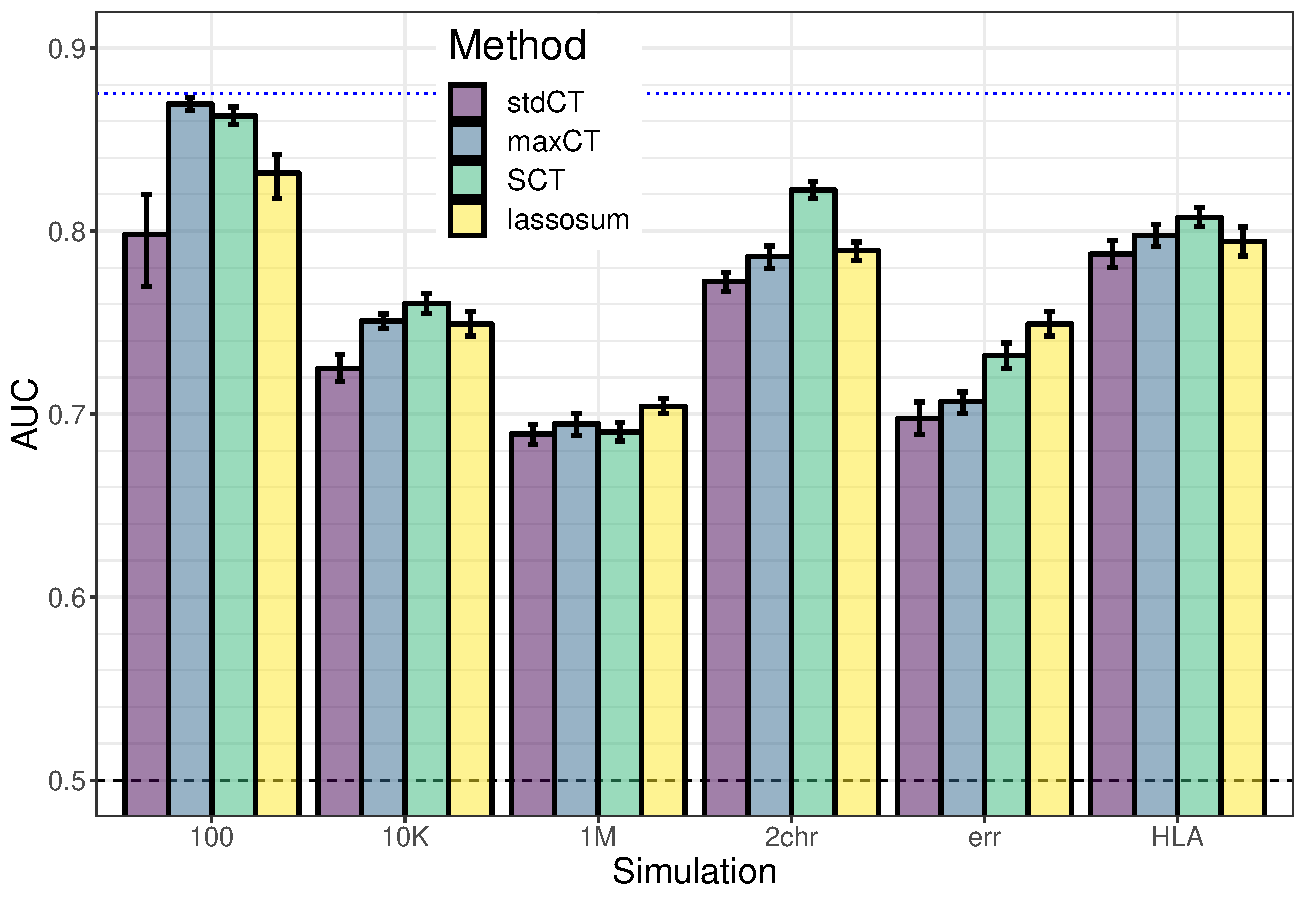
\includegraphics[width=0.8\textwidth]{AUC-simus.pdf}}
\caption{Results of the 6 simulation scenarios: (100) 100 random causal SNPs; (10K) 10,000 random causal SNPs; (1M) all 1M SNPs are causal SNPs; (2chr) 100 SNPs of chromosome 1 are causal and all SNPs of chromosome 2, with half of the heritability for both chromosomes; (err) 10,000 random causal SNPs, but 10\% of the GWAS effects are reported with an opposite effect; (HLA) 7105 causal SNPs in a long-range LD region of chromosome 6. Mean and 95\% CI of $10^4$ non-parametric bootstrap replicates of the mean AUC of 10 simulations for each scenario. The blue dotted line represents the maximum achievable AUC for these simulations (87.5\% for a prevalence of 10\% and an heritability of 50\% -- see equation (3) of \cite{wray2010genetic}).}
\label{fig:AUC-simus}
\end{figure}

As for SCT, it provides equal or higher predictive performance than maxCT in simulation scenarios (Figure \ref{fig:AUC-simus}). In the first three simple scenarios simulating 100, 10K or 1M causal SNPs anywhere on the genome, predictive performance of SCT are similar to maxCT. In the ``2chr'' scenario where there are large effects on chromosome 1, small effects on chromosome 2 and no effect on other chromosomes, mean AUC is 78.7\% for maxCT and 82.2\% for SCT, which is an absolute increase of 3.5\%. In the ``err'' scenario where we report GWAS summary statistics with 10\% reversed effects (errors), mean AUC is 70.2\% for maxCT and 73.2\% for SCT, which is an absolute increase of 3\%.

[DESCRIBE PLOTS OF EFFECTS?]


\subsection{Real summary statistics}

In terms of AUC, maxCT outperfoms stdCT and  for all 8 diseases consireded with a mean absolute increase of 1.3\% (Figure \ref{fig:AUC-real} and table \ref{tab:AUC}). 
A particularly large increase can be noted when predicting depression status (MDD), from an AUC of 55.7\% (95\% CI: [54.4-56.9]) with stdCT to an AUC of 59.2\% (95\% CI: [58.0-60.4]) with maxCT. For MDD, a liberal inclusion in clumping ($r_c^2$ = 0.8) and a stringent threshold on imputation accuracy ($\text{INFO}_T$ = 0.95) provides the best predictive performance (Figure \ref{fig:grid-MDD}).
For all 8 diseases, predictions were optimized when choosing a threshold on imputation accuracy of at least 0.9, whereas optimal values for $r_c^2$ where very different depending on the architecture of diseases, with optimal selected values over the whole range of tested values for $r_c^2$ (Table \ref{tab:param}).

\begin{figure}[h]
\centerline{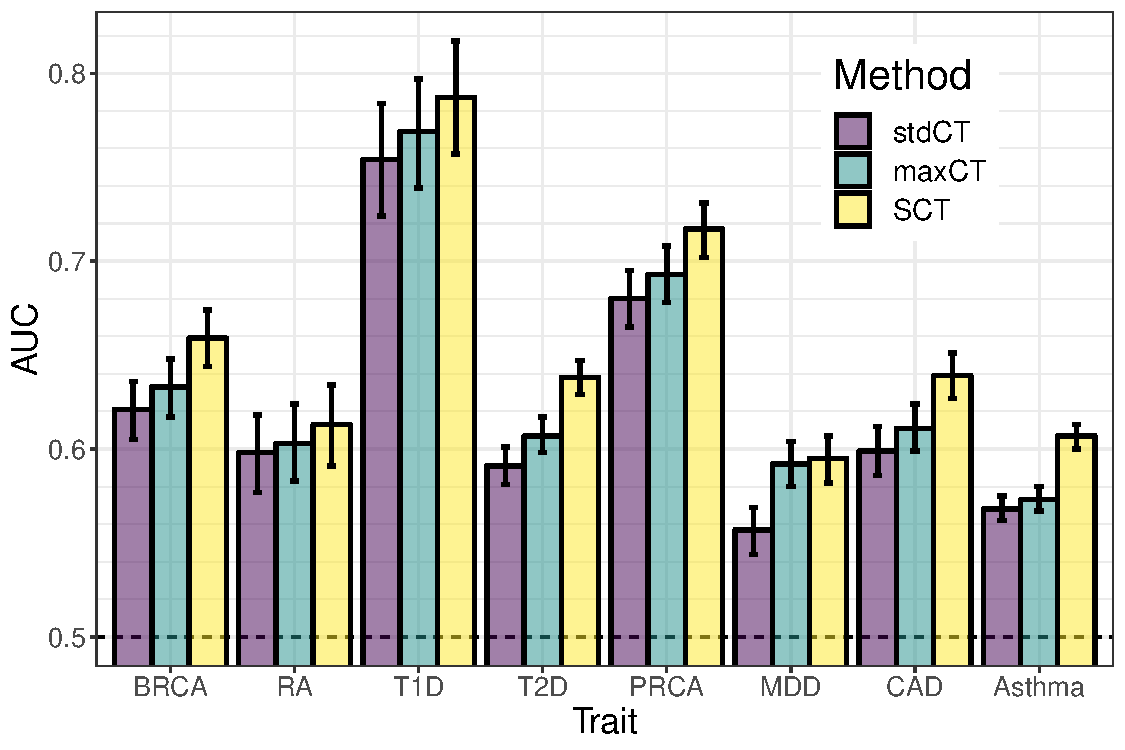
\includegraphics[width=0.8\textwidth]{AUC-real.pdf}}
\caption{AUC values on the test set of UKBB (mean and 95\% CI from $10^4$ bootstrap samples). See corresponding values in table \ref{tab:AUC}.}
\label{fig:AUC-real}
\end{figure}

Furthermore, SCT outforms maxCT for all 8 diseases consireded with an additional mean absolute increase of AUC of 2.2\%, making it 3.5\% as compared to stdCT (Figure \ref{fig:AUC-real} and table \ref{tab:AUC}).
Predictive performance improvement of SCT versus maxCT is particularly notable for prostate cancer (2.4\%), breast cancer (2.6\%), coronary artery disease (2.8\%), type 2 diabetes (3.1\%) and asthma (3.4\%).

Effects resulting from SCT have mostly the same sign as initial effects from GWAS, with few effects being largely unchanged, and others having an effect that is shrunk to 0 or completely 0, i.e.\ variants not included in the final model (Figure \ref{fig:neweffreal}).

[WHAT ELSE?]

%%%%%%%%%%%%%%%%%%%%%%%%%%%%%%%%%%%%%%%%%%%%%%%%%%%%%%%%%%%%%%%%%%%%%%%%%%%%%%%%

\section{Discussion}

\subsection{Predictive performance improvement of C+T}

C+T is a widely-used method for computing PRS. 
C+T is considered as a simple technique because it directly uses effects from GWAS regression coefficients and that it simply discards SNPs in LD instead of accounting for LD in a more optimal way \cite[]{vilhjalmsson2015modeling}. 
The popularity of this method may be due to both PLINK and PRSice, two pieces of software that make it easy to apply C+T \cite[]{purcell2007plink,euesden2014prsice,chang2015second}.

In this paper, we show that this method has at least 4 hyper-parameters to choose (minor allele frequency might be a fifth one) and we provide some efficient software to compute C+T scores for many combinations of these parameters.
Using simulated and real data, we show that choosing different values rather than default ones for these hyper-parameters has the potential to substantially improves performance of C+T.
We cannot test all possible combinations of these parameters, but it is possible to rerun the method using a finer grid in a particular range of these hyper-parameters. For example, it might be useful to include SNPs with p-values larger than 0.1 for predicting rheumatoid arthritis and depression (Figures \ref{fig:grid-RA} and \ref{fig:grid-MDD}). Another example would be to focus on a finer grid of large values of $r_c^2$ for coronary artery disease (Figure \ref{fig:grid-CAD}).

Using this large grid of C+T scores for many different hyper-parameters, we show that stacking these scores instead of choosing the best one improves prediction further \cite[]{breiman1996stacked}.
You may see SCT as a metaGRS pushed to the limit \cite[]{inouye2018genomic}.
Normally, cross-validation should be used to prevent overfitting when using stacking and it is also suggested to use positivity constraints in stacking \cite[]{breiman1996stacked}.
However, cross-validation is not necessary here since building C+T scores does not make use of the phenotype of the training set that is later used in the stacking.
Moreover, we allow C+T scores to have negative weights in the final model. We think it makes sense to do so for three reasons. First, because C+T scores are overlapping, negative weights makes it possible to only weight groups of SNPs that are ``in the middle''. Second, because of LD, some SNPs might have different effects when learned jointly with others (Figures \ref{fig:neweff1M} and \ref{fig:neweffHLA}). Third, if reported GWAS effects are merely different in the data we compute the PRS, for example when applying SCT in different population as the GWAS,  having SNPs with opposite effects might help adapting the GWAS effects (Figure \ref{fig:newefferr}).
[NOT SO CLEAR..]

\subsection{Limitations of the study}

We analyze 8 different binary phenotypes in this study, but there are more to be analyzed. For example, for psychiatric disease, we include only depression (MDD) because diseases such as schyzophrenia and bipolar disorder have very few cases in the UK Biobank; dedicated datasets should be used to assess effectiveness of maxCT and SCT for such diseases. 
We also do not analyze many automimmune diseases as summary statistics are often outdated\footnote{https://www.immunobase.org/downloads/protected\_data/GWAS\_Data/} and, because there are usually large effects on chromosome 6, methods that use individual-level data instead of summary statistics are likely to provide better predictive models \cite[]{prive2019efficient}.
We also voluntarily do not analyze any continuous trait such as height or BMI because there are many individual-level data available for such phenotypes and methods directly using individual-level data are likely to provide better predictive models than the ones using summary statistics \cite[]{prive2019efficient}. 
Phenotypes with tiny effects such as educational attainment for which huge GWAS summary statistics are available might be an exception \cite[]{lee2018gene}.

Moreover, we focus this study on improving the C+T method. The C+T method is by far the simplest and most widely-used method for constructing polygenic risk scores based on summary statistics. The idea behind C+T is really simple because it directly uses weights learned from GWAS; it further removes SNPs as one does when reporting hits from GWAS, i.e.\ only SNPs that pass the genome-wide threshold (p-value thresholding) and that are independent association findings (clumping) are reported. 
Yet, there are two other established methods based on summary statistics, LDpred and lassosum \cite[]{vilhjalmsson2015modeling,mak2017polygenic,allegrini2019genomic}. Several other recent methods such as NPS, PRS-CS and SBayesR are being developed \cite[]{chun2019non,ge2019polygenic,lloyd2019improved}.
Some methods require only a small reference panel to account for LD while some methods have a phase of retraining that needs a training set with individual-level data and phenotypes (SCT, NPS and lassosum).
A full comparison of methods (including individual-level data methods), including binary and continuous traits with different architectures, using different sizes of summary statistics and individual-level data for training, and in possibly different populations would make a fantastic paper. 
Indeed, we believe that different methods may perform very differently in different settings and that understanding in which case which method works best is a key need if we want to maximize the utility of PRS.


\subsection{Areas of improvement}

There are many ways to improve prediction further. For example, developing techniques that can handle errors should be of great interest \cite[]{smith2011improving,bolin2014supervised}. There are many applications in medical data.
First, there can be mistakes in meta-analyses results \cite[]{greco2013meta}, mistakes in disease diagnostic \cite[]{wray2012impact,thomas2018frequency}, imprecisions in data, or defining ambiguous alleles \cite[]{chen2018prs}. [MORE DETAILS + REFS]
For example, in one simulation scenario (``err'') of this paper, we show that having an extra layer of training consisting in stacking C+T models makes it possible to partially correct for mistakes.

As for the SCT method itself, the stacking step can be used for either binary or continuous phenotypes. 
Yet, it makes sense to use age in the models, using for example Cox proportional-hazards model to predict age of disease onset, with possibly censored data \cite[]{cox1972regression}.
Cox regression has already proven useful for increasing power in GWAS \cite[]{hughey2019cox}.
Cox model is not implemented yet as part as our efficient penalized regression implementation, only linear and logistic regressions are. This is an area of future development; at the moment, if sample size is not too large, one could use R package glmnet to implement stacking based on Cox model \cite[]{tibshirani2012strong}.

One might also want to use other information such as sex or ancestry (using principal components). Indeed, it is easy to add those in the stacking step as (unpenalized) variables in the penalized logistic regression. Yet, we have to be cautious doing so. For example, because prevalence of CAD is much higher in men than in women in the UKBB (8-9\% vs 2\%), adding sex in the model amount to fitting two different intercepts, centering distributions of fitted probabilities around disease prevalence (Figure \ref{fig:sexCAD}). This increases the AUC from 63.9\% to 74.4\% but results in a model that would classify all women as healthy. A possible solution would be to report AUC figures for each gender separately, or even to fit a model for each gender separately (in the stacking step).
Fitting models separately would enable the use of sex chromosomes without introducing bias. 
As for ancestry concerns, fitting different models for different ancestries might be a way to get more calibrated results and to account for differences in effect sizes and LD. 
However, here for CAD, fitting two separate models results in a slight loss of predictive performance, while using variable `sex' does not change results when they are reported for each gender separately, with an AUC of 64.9\% [63.5-66.3] for men and 62.5\% [59.8-65.2] for women.
Thus, adding `sex' as a covariate in the model may provide a model with similar discrimination and with better calibration of probabilities (if prevalence in the data is representative of prevalence in the population). Yet, we would like to emphasize again that reporting one AUC figure for all individuals would be misleading in the case of using variable `sex' in the model.


\subsection{Conclusion}

We focus this paper on improving the widely-used C+T method by testing a wide-range of hyper-parameters values. More broadly, we believe that any implementation of statistical methods should come with an easy and effective way to choose hyper-parameters of these methods well. 
We believe that C+T will continue to be used for many years as it is both simple to use and to understand. 
Moreover, it remains an effective method since it can adapt to many different disease architectures by choosing hyper-parameters well.
Instead of choosing one set of hyper-parameters, we show that stacking C+T predictions further improves predictive performance. 
There are many advantages of SCT over any single C+T prediction: first, it can learn different architecture models for different chromosomes, it can learn a mixture of large and small effects and it can more generally adapt initial weights of the GWAS in order to maximize prediction.
Moreover, model resulting from SCT, as a linear combination (stacking) of linear combinations (C+T scores), it remains a simple linear model with one vector of coefficients. 
As logistic regression is used for stacking C+T scores for binary traits, resulting predictions returns probabilities, if one needs usually better calibrated models. [REWORD]

[WHAT ELSE?]

%%%%%%%%%%%%%%%%%%%%%%%%%%%%%%%%%%%%%%%%%%%%%%%%%%%%%%%%%%%%%%%%%%%%%%%%%%%%%%%%

\newpage

\section*{Acknowledgements}

Authors acknowledge LabEx PERSYVAL-Lab (ANR-11-LABX-0025-01) and ANR project FROGH (ANR-16-CE12-0033). Authors also acknowledge the Grenoble Alpes Data Institute that is supported by the French National Research Agency under the ``Investissements d'avenir'' program (ANR-15-IDEX-02).
This research has been conducted using the UK Biobank Resource under Application Number 25589.

%%%%%%%%%%%%%%%%%%%%%%%%%%%%%%%%%%%%%%%%%%%%%%%%%%%%%%%%%%%%%%%%%%%%%%%%%%%%%%%%

\newpage

\bibliographystyle{natbib}
\bibliography{refs}

%%%%%%%%%%%%%%%%%%%%%%%%%%%%%%%%%%%%%%%%%%%%%%%%%%%%%%%%%%%%%%%%%%%%%%%%%%%%%%%%

\newpage
\section*{Supplementary Data}

\renewcommand{\thefigure}{S\arabic{figure}}
\setcounter{figure}{0}
\renewcommand{\thetable}{S\arabic{table}}
\setcounter{table}{0}

\begin{figure}[htb]
\centerline{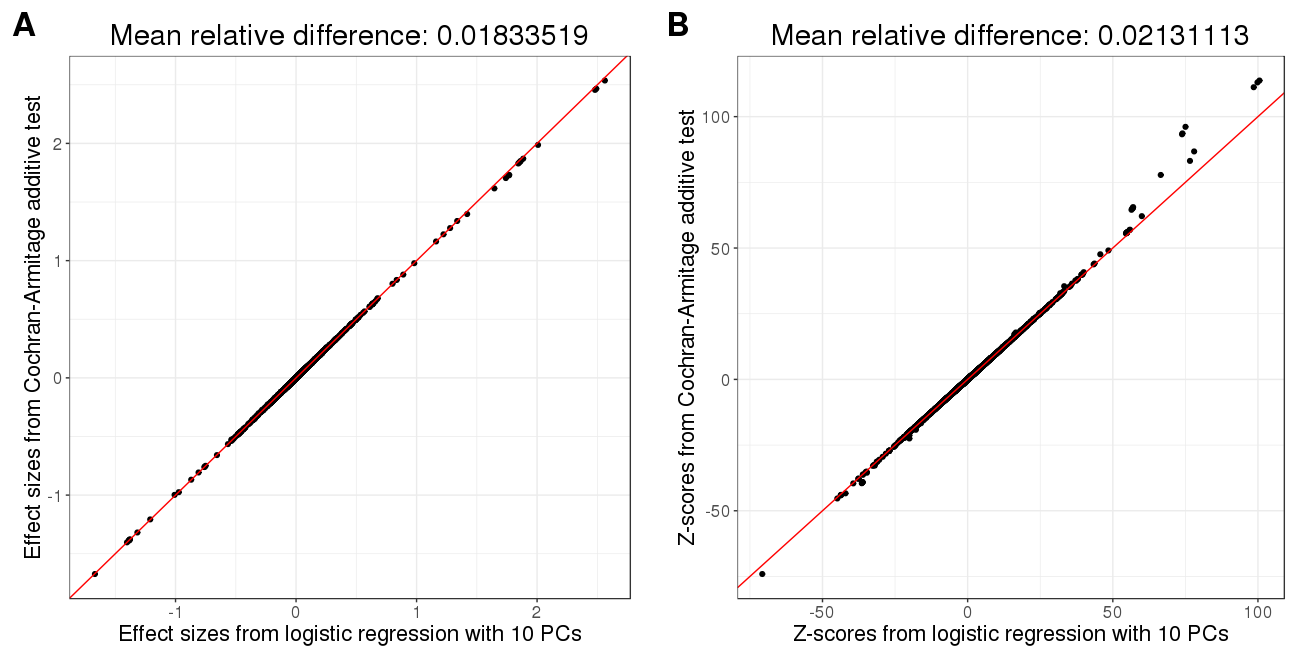
\includegraphics[width=0.95\textwidth]{equivalence.png}}
\caption{Comparison of estimated effect sizes (\textbf{A}) and Z-scores (\textbf{B}) if computed using a logistic regression with 10 principal components as covariates, or with a simple Cochran-Armitage additive test. Phenotypes were simulated using 100 causal SNPs only, allowing for large effects.}
\label{fig:GWAS}
\end{figure}

%%%%%%%%%%%%%%%%%%%%%%%%%%%%%%%%%%%%%%%%%%%%%%%%%%%%%%%%%%%%%%%%%%%%%%%%%%%%%%%%

\begin{table}[h]
\caption{AUC values on the test set of UKBB (mean [95\% CI] from $10^4$ bootstrap samples) and the number of variants used in the final model.\label{tab:AUC}}
\vspace*{0.5em}
\centering
\begin{tabular}{|l|c|c|c|c|}
  \hline
Trait & stdCT & maxCT & SCT \\
  \hline
Breast cancer (BRCA) & 62.1 [60.5-63.6] & 63.3 [61.7-64.8] & 65.9 [64.4-67.4] \\
 & 6256 & 2572 & 670,050 \\
Rheumatoid arthritis (RA) & 59.8 [57.7-61.8] & 60.3 [58.3-62.4] & 61.3 [59.1-63.4] \\
 & 12,220 & 88,556 & 317,456 \\
Type 1 diabetes (T1D) & 75.4 [72.4-78.4] & 76.9 [73.9-79.7] & 78.7 [75.7-81.7] \\
 & 1112 & 267 & 135,991 \\
Type 2 diabetes (T2D) & 59.5 [58.5-60.5] & 60.7 [59.8-61.6] & 63.8 [62.9-64.8] \\
 & 252 & 33,238 & 535,785 \\
Prostate cancer (PRCA) & 68.0 [66.5-69.5] & 69.3 [67.8-70.8] & 71.7 [70.2-73.1] \\
 & 1035 & 356 & 696,575 \\
Depression (MDD) & 55.7 [54.4-56.9] & 59.2 [58.0-60.4] & 59.5 [58.2-60.7] \\
 & 165,584 & 222,912 & 524,099 \\
Coronary artery disease (CAD) & 59.9 [58.6-61.2] & 61.1 [59.9-62.4] & 63.9 [62.7-65.1] \\
 & 1182 & 87,577 & 315,165 \\
Asthma & 56.8 [56.2-57.5] & 57.3 [56.7-58.0] & 60.7 [60.0-61.3] \\
 & 3034 & 360 & 446,120 \\
   \hline
\end{tabular}
\end{table}

%%%%%%%%%%%%%%%%%%%%%%%%%%%%%%%%%%%%%%%%%%%%%%%%%%%%%%%%%%%%%%%%%%%%%%%%%%%%%%%%

\begin{table}[h]
\caption{Choice of C+T parameters based on the maximum AUC in the training set.\label{tab:param}}
\vspace*{0.5em}
\centering
\begin{tabular}{|l|c|c|c|c|c|}
  \hline
Trait & $w_c$ & $r_c^2$ & $\text{INFO}_T$ & $p_T$ \\
  \hline
Breast cancer (BRCA)          & 2500    & 0.2  & 0.95 & 2.2e-04 \\
Rheumatoid arthritis (RA)     & 200     & 0.5  & 0.95 & 7.5e-02 \\
Type 1 diabetes (T1D)         & 10K-50K & 0.01 & 0.90 & 2.6e-05 \\
Type 2 diabetes (T2D)         & 625     & 0.8  & 0.95 & 1.1e-02 \\
Prostate cancer (PRCA)        & 10K-50K & 0.01 & 0.90 & 4.2e-06 \\
Depression (MDD)              & 625     & 0.8  & 0.95 & 1.0e-01 \\
Coronary artery disease (CAD) & 526     & 0.95 & 0.95 & 3.5e-02 \\
Asthma                        & 2500    & 0.2  & 0.90 & 2.2e-04 \\
   \hline
\end{tabular}
\end{table}

%%%%%%%%%%%%%%%%%%%%%%%%%%%%%%%%%%%%%%%%%%%%%%%%%%%%%%%%%%%%%%%%%%%%%%%%%%%%%%%%

\begin{figure}[htb]
\centering
\begin{subfigure}[b]{0.7\textwidth}
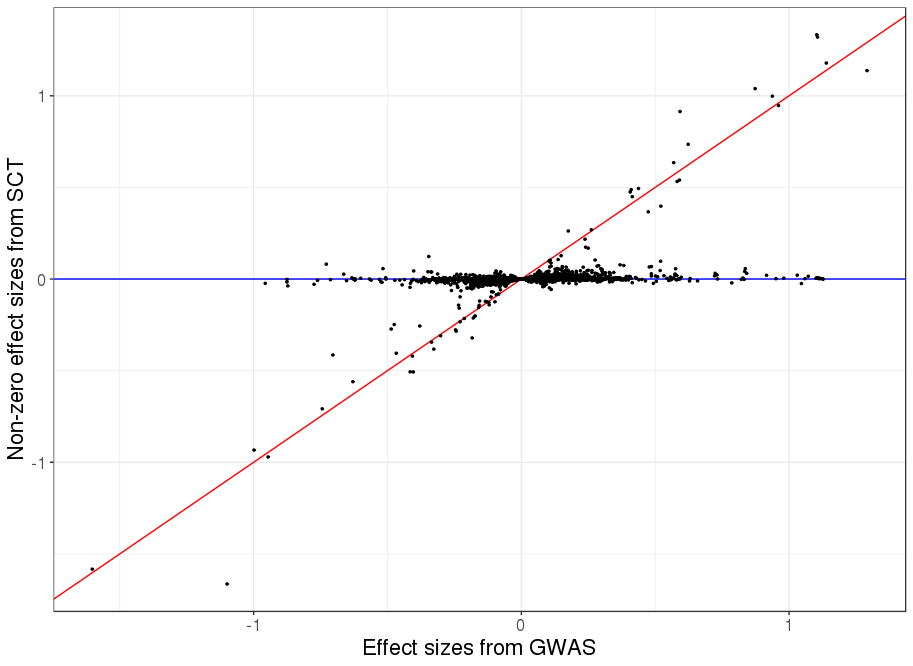
\includegraphics[width=\textwidth]{new-effects-simu100.png}
\caption{100 random causal SNPs}
\end{subfigure}
\\~\\~\\
\begin{subfigure}[b]{0.7\textwidth}
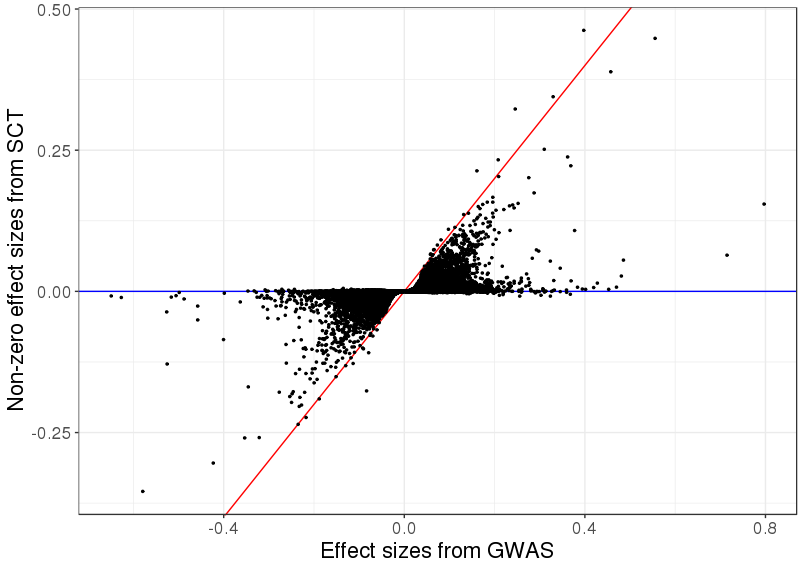
\includegraphics[width=\textwidth]{new-effects-simu10K.png}
\caption{10,000 random causal SNPs}
\end{subfigure}
\end{figure}

\begin{figure}[htb]\ContinuedFloat
\centering
\begin{subfigure}[b]{0.7\textwidth}
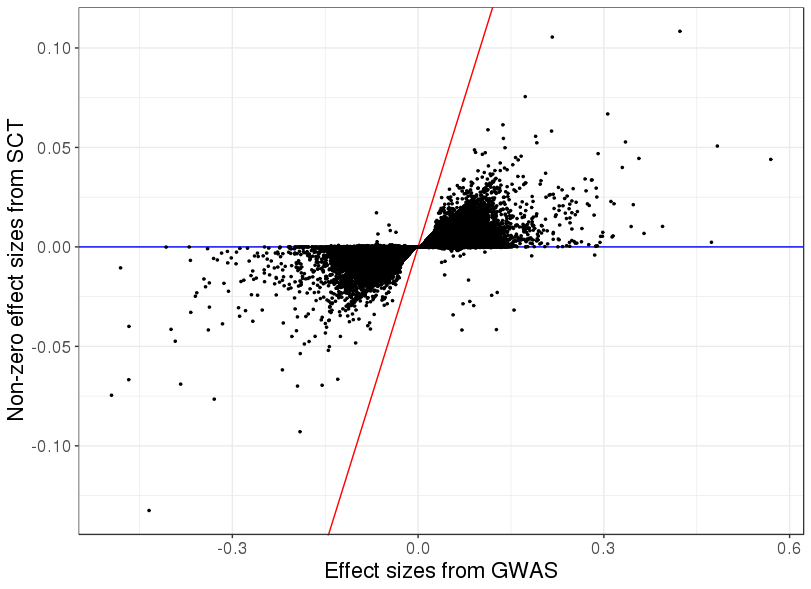
\includegraphics[width=\textwidth]{new-effects-simu1M.png}
\caption{all 1M SNPs are causal SNPs\label{fig:neweff1M}}
\end{subfigure}
\\~\\~\\
\begin{subfigure}[b]{0.7\textwidth}
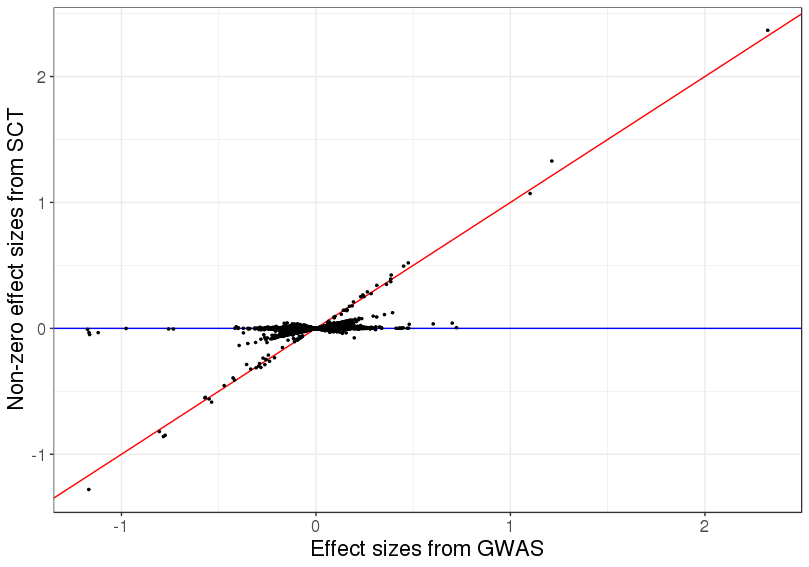
\includegraphics[width=\textwidth]{new-effects-simu2chr.png}
\caption{Causal SNPs on chromosomes 1 \& 2}
\end{subfigure}
\end{figure}

\begin{figure}[htb]\ContinuedFloat
\centering
\begin{subfigure}[b]{0.7\textwidth}
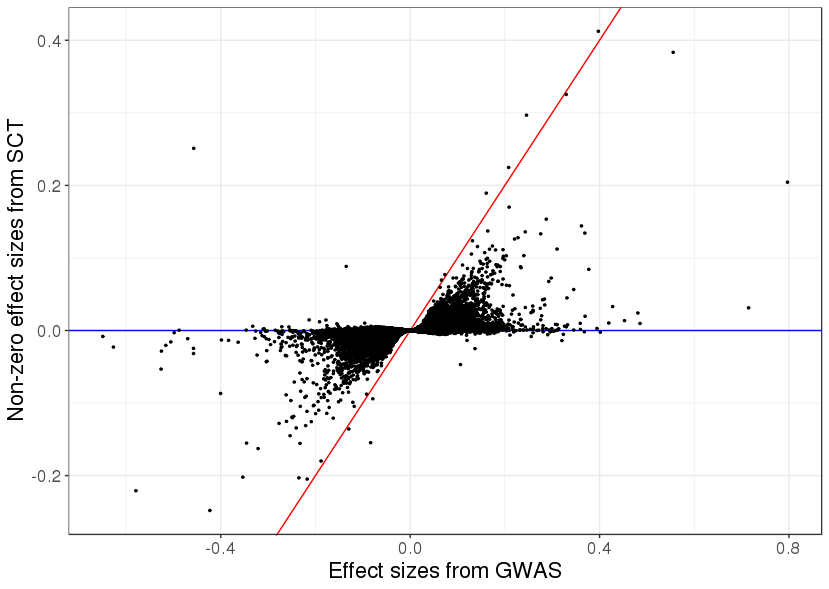
\includegraphics[width=\textwidth]{new-effects-simuerr.png}
\caption{10,000 random causal SNPs, but 10\% of the GWAS effects are reported with an opposite effect\label{fig:newefferr}}
\end{subfigure}
\\~\\~\\
\begin{subfigure}[b]{0.7\textwidth}
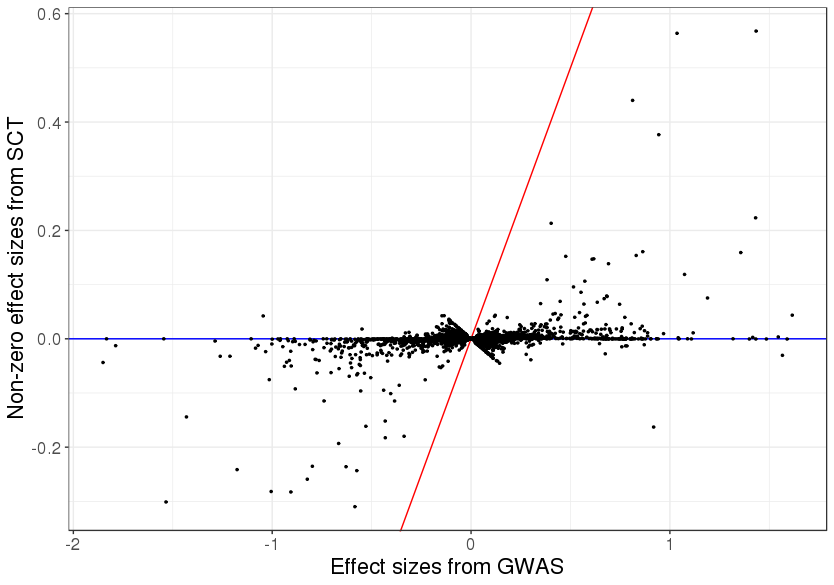
\includegraphics[width=\textwidth]{new-effects-simuHLA.png}
\caption{7105 causal SNPs in a long-range LD region of chromosome 6.\label{fig:neweffHLA}}
\end{subfigure}

\caption{New effect sizes resulting from SCT versus initial effect sizes of GWAS in the first simulation of each simulation scenario. Only non-zero effects are represented. Red line corresponds to the 1:1 line.}
\label{fig:neweffsimu}
\end{figure}

%%%%%%%%%%%%%%%%%%%%%%%%%%%%%%%%%%%%%%%%%%%%%%%%%%%%%%%%%%%%%%%%%%%%%%%%%%%%%%%%

\begin{figure}[htb]
\centering
\begin{subfigure}[b]{\textwidth}
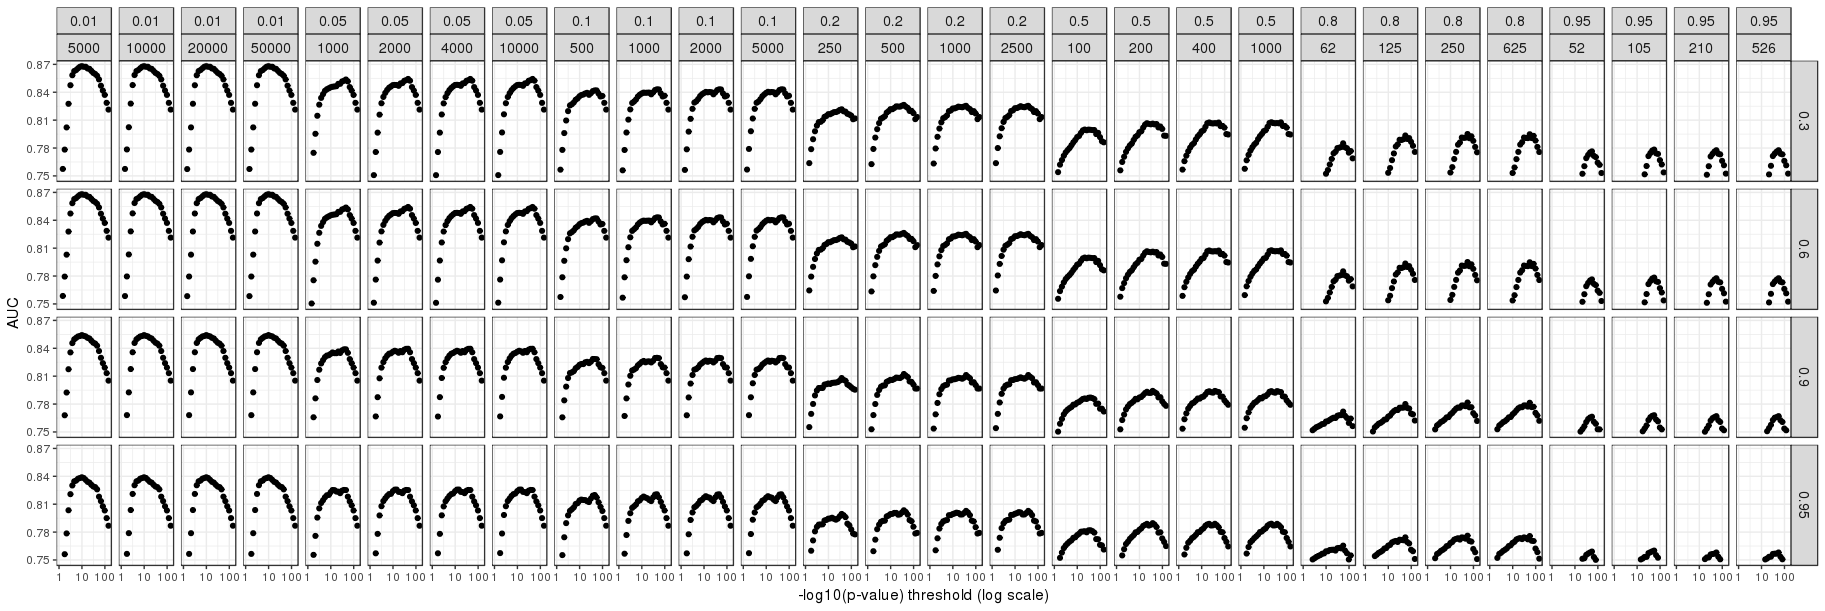
\includegraphics[width=\textwidth]{grid-simu100.png}
\caption{100 random causal SNPs\label{fig:simugridA}}
\end{subfigure}
\\~\\~\\
\begin{subfigure}[b]{\textwidth}
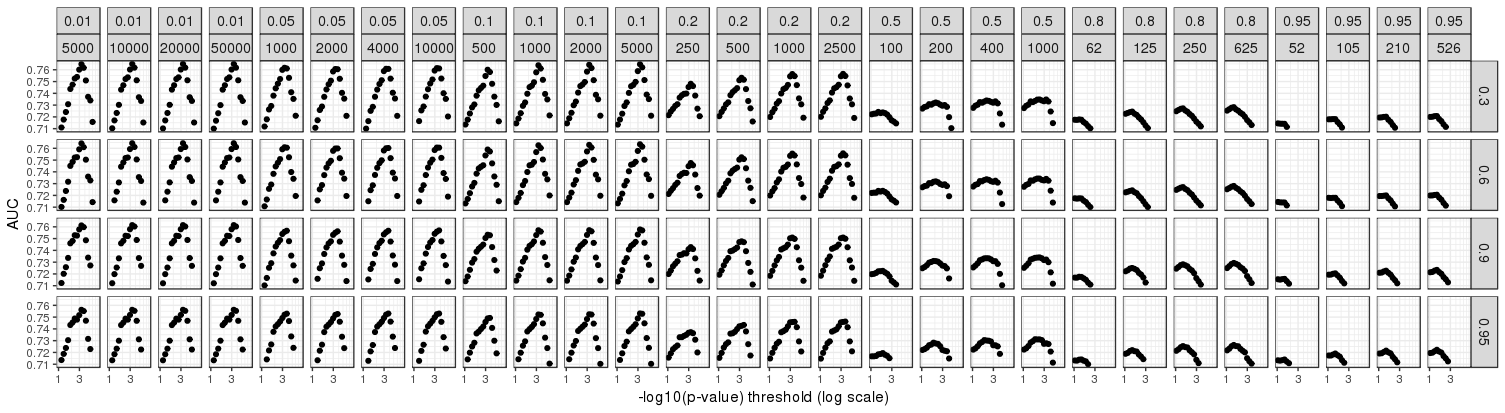
\includegraphics[width=\textwidth]{grid-simu10K.png}
\caption{10,000 random causal SNPs\label{fig:simugridB}}
\end{subfigure}
\\~\\~\\
\begin{subfigure}[b]{\textwidth}
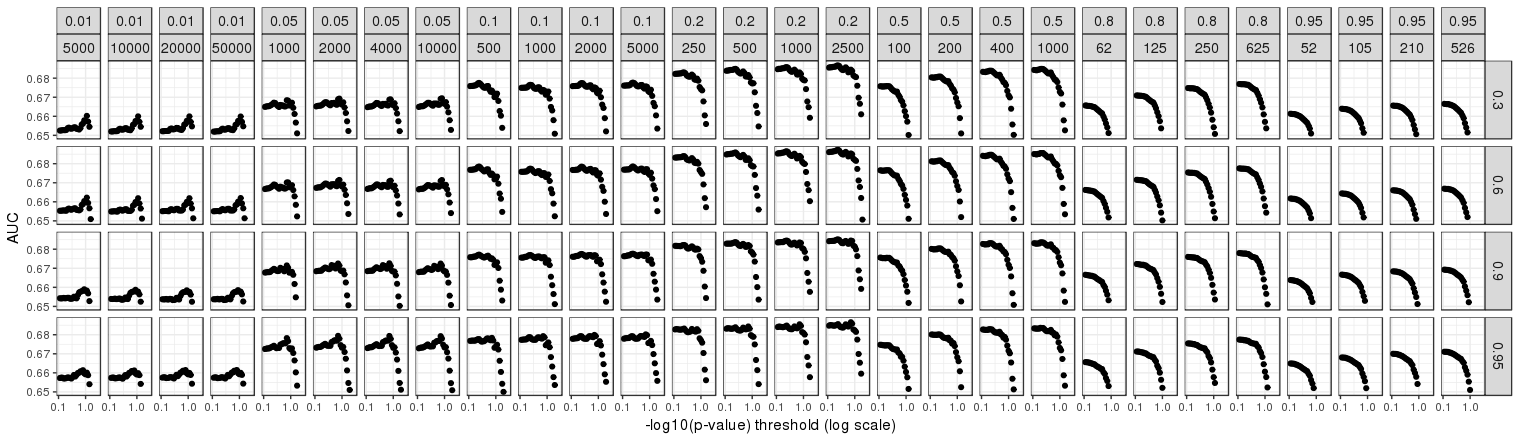
\includegraphics[width=\textwidth]{grid-simu1M.png}
\caption{all 1M SNPs are causal SNPs\label{fig:simugridC}}
\end{subfigure}
\end{figure}

\begin{figure}[htb]\ContinuedFloat
\centering
\begin{subfigure}[b]{\textwidth}
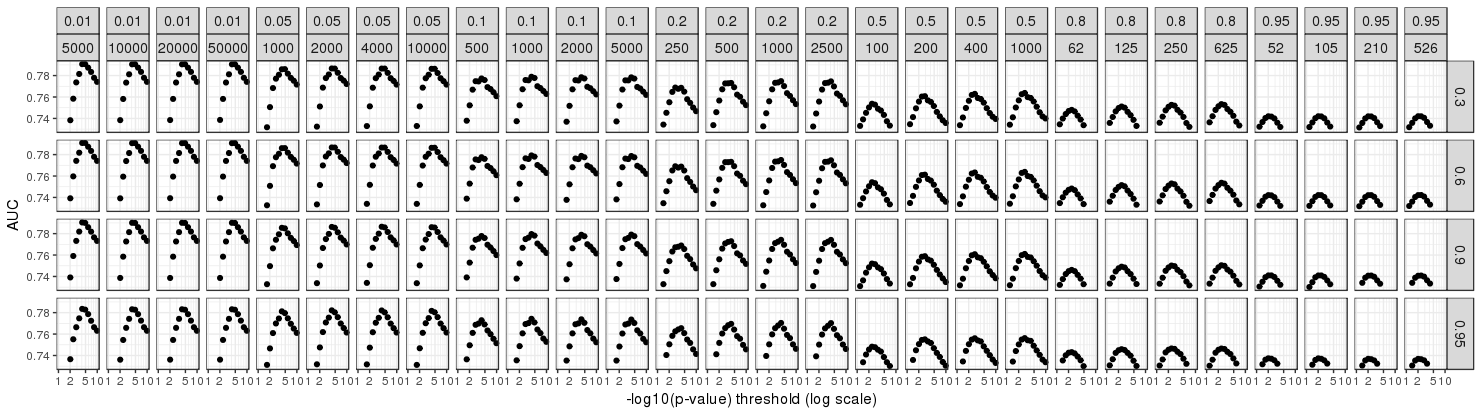
\includegraphics[width=\textwidth]{grid-simu2chr.png}
\caption{Causal SNPs on chromosomes 1 \& 2}
\end{subfigure}
\\~\\~\\
\begin{subfigure}[b]{\textwidth}
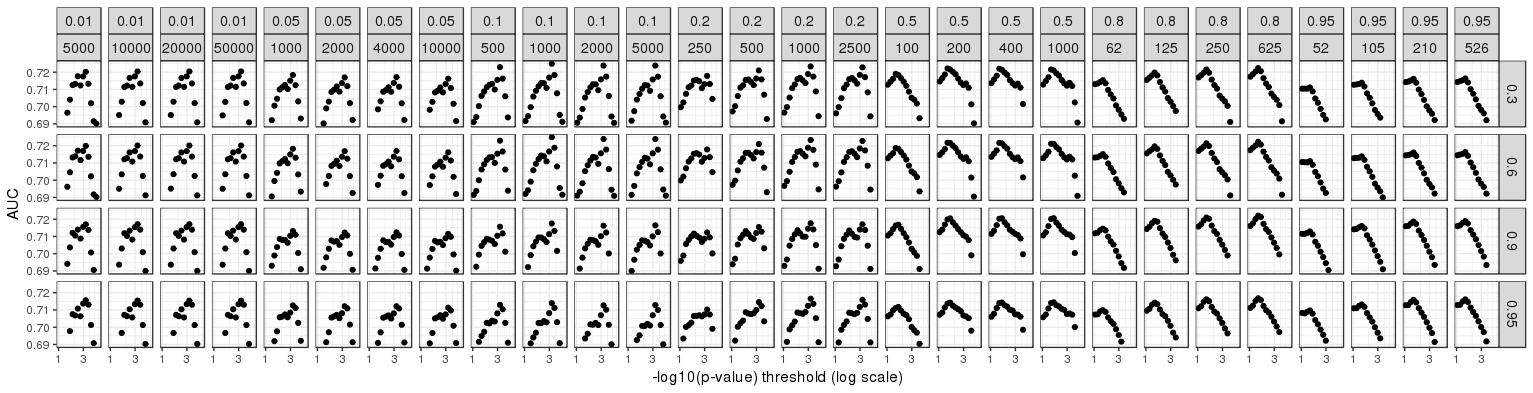
\includegraphics[width=\textwidth]{grid-simuerr.png}
\caption{10,000 random causal SNPs, but 10\% of the GWAS effects are reported with an opposite effect}
\end{subfigure}
\\~\\~\\
\begin{subfigure}[b]{\textwidth}
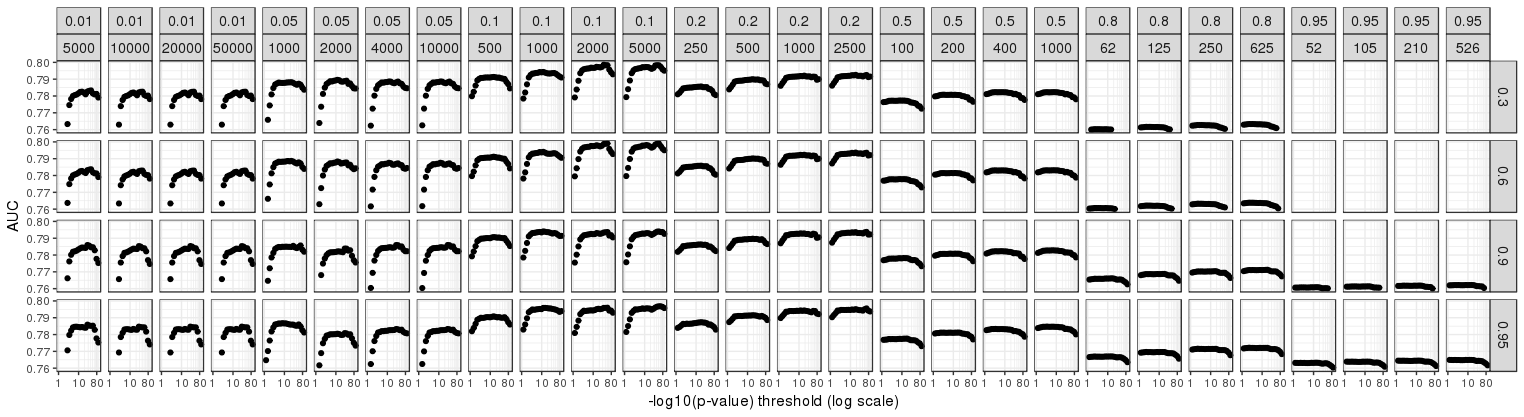
\includegraphics[width=\textwidth]{grid-simuHLA.png}
\caption{7105 causal SNPs in a long-range LD region of chromosome 6.}
\end{subfigure}

\caption{AUC values (for the training set) when predicting disease status for many parameters of C+T in the first simulation of each simulation scenario. Facets are presenting different clumping thresholds $r_c^2$ from 0.01 to 0.95, window sizes $w_c$ from 52 to 50,000 kb, and imputation thresholds from 0.3 to 0.95. The x-axis corresponds to the remaining hyper-parameter, the p-value threshold $p_T$; here, -log10(p-values) are represented using a logarithmic scale.}
\end{figure}

%%%%%%%%%%%%%%%%%%%%%%%%%%%%%%%%%%%%%%%%%%%%%%%%%%%%%%%%%%%%%%%%%%%%%%%%%%%%%%%%

\begin{figure}[htb]
\centering
\begin{subfigure}[b]{0.7\textwidth}
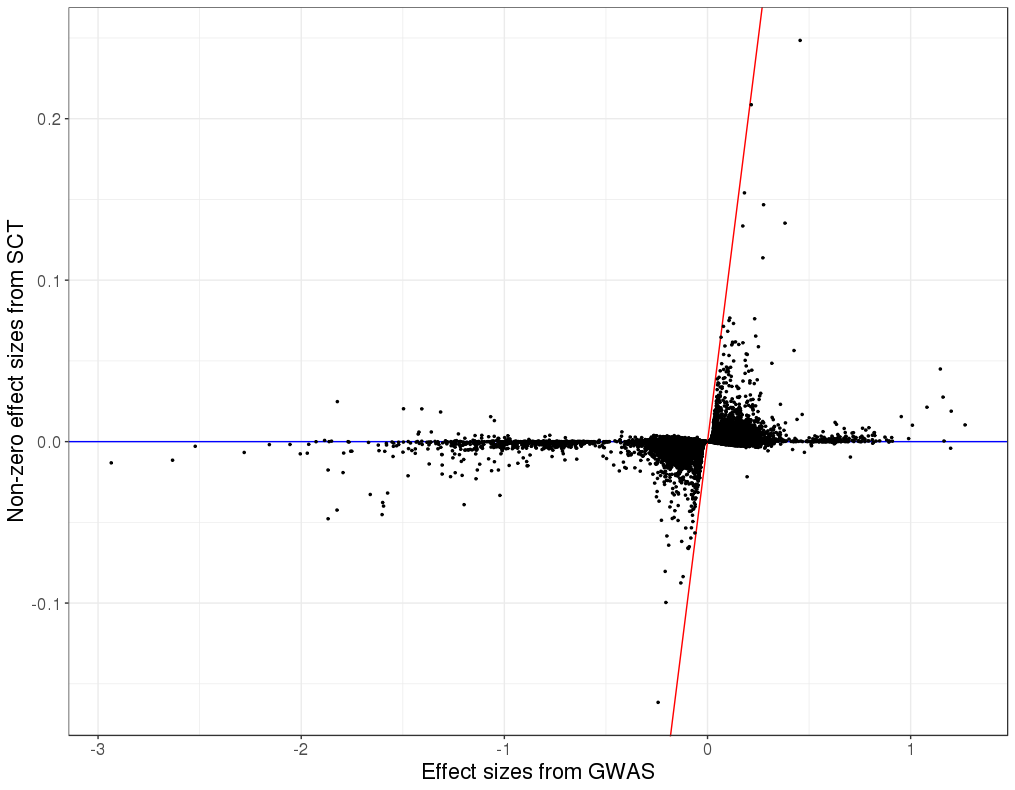
\includegraphics[width=\textwidth]{new-effects-BRCA.png}
\caption{Breast cancer}
\end{subfigure}
\\~\\~\\
\begin{subfigure}[b]{0.7\textwidth}
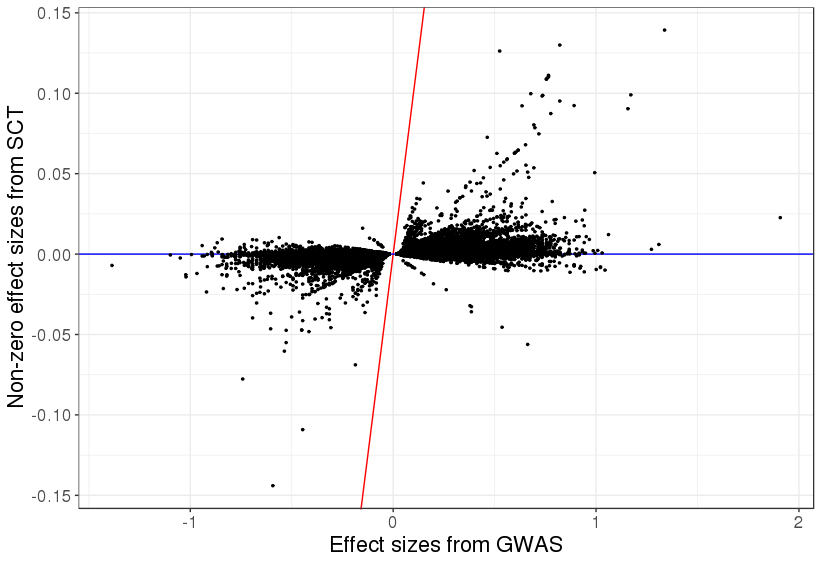
\includegraphics[width=\textwidth]{new-effects-RA.png}
\caption{Rheumatoid arthritis}
\end{subfigure}
\end{figure}

\begin{figure}[htb]\ContinuedFloat
\centering
\begin{subfigure}[b]{0.7\textwidth}
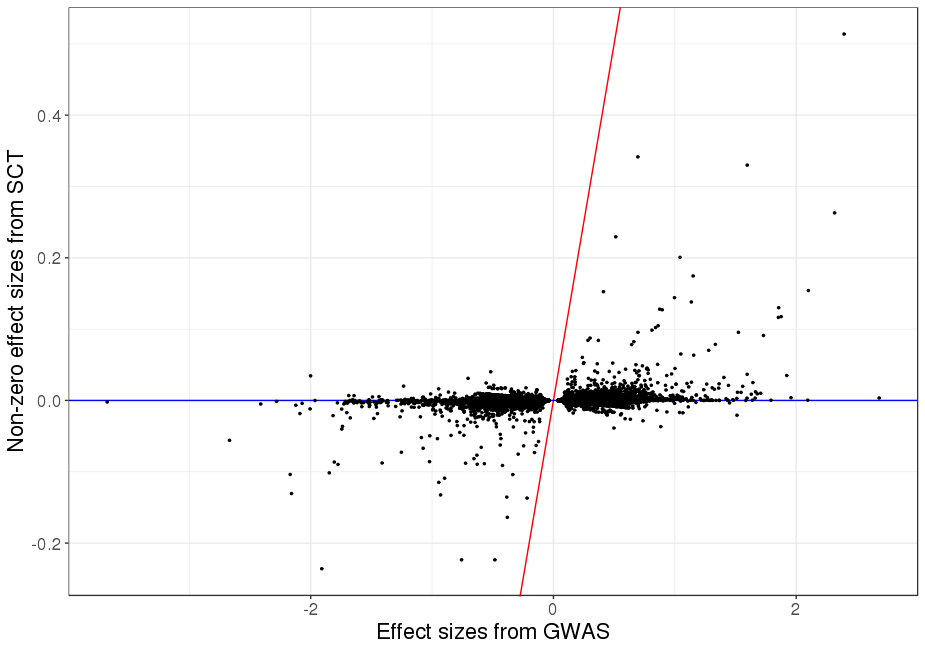
\includegraphics[width=\textwidth]{new-effects-T1D.png}
\caption{Type 1 diabetes}
\end{subfigure}
\\~\\~\\
\begin{subfigure}[b]{0.7\textwidth}
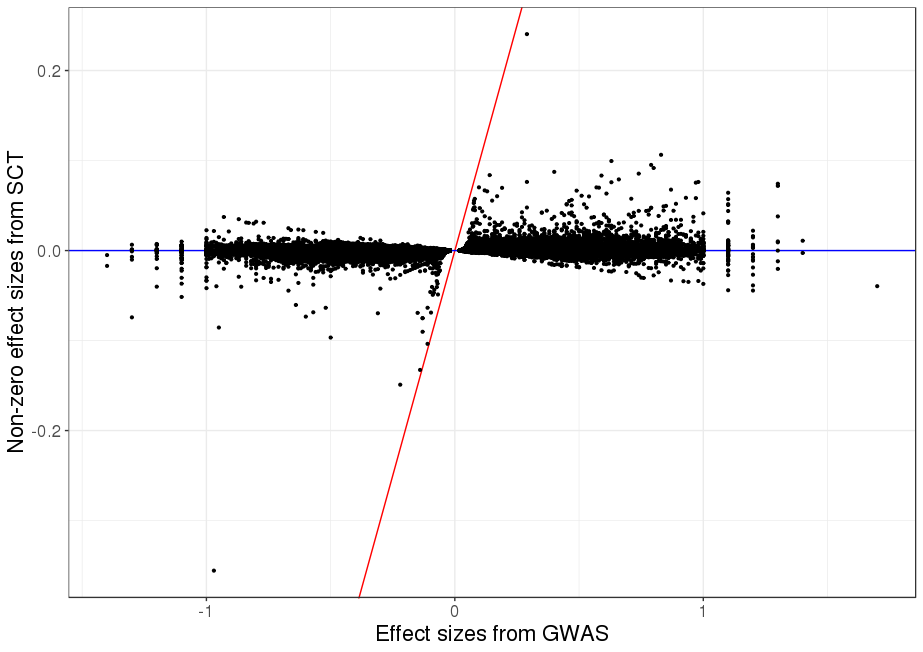
\includegraphics[width=\textwidth]{new-effects-T2D.png}
\caption{Type 2 diabetes}
\end{subfigure}
\end{figure}

\begin{figure}[htb]\ContinuedFloat
\centering
\begin{subfigure}[b]{0.7\textwidth}
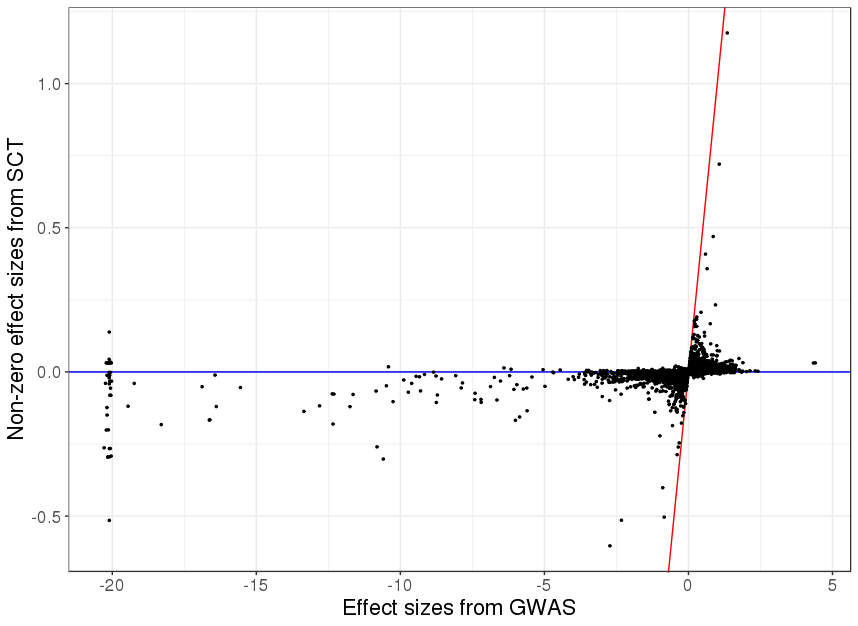
\includegraphics[width=\textwidth]{new-effects-PRCA.png}
\caption{Prostate cancer}
\end{subfigure}
\\~\\~\\
\begin{subfigure}[b]{0.7\textwidth}
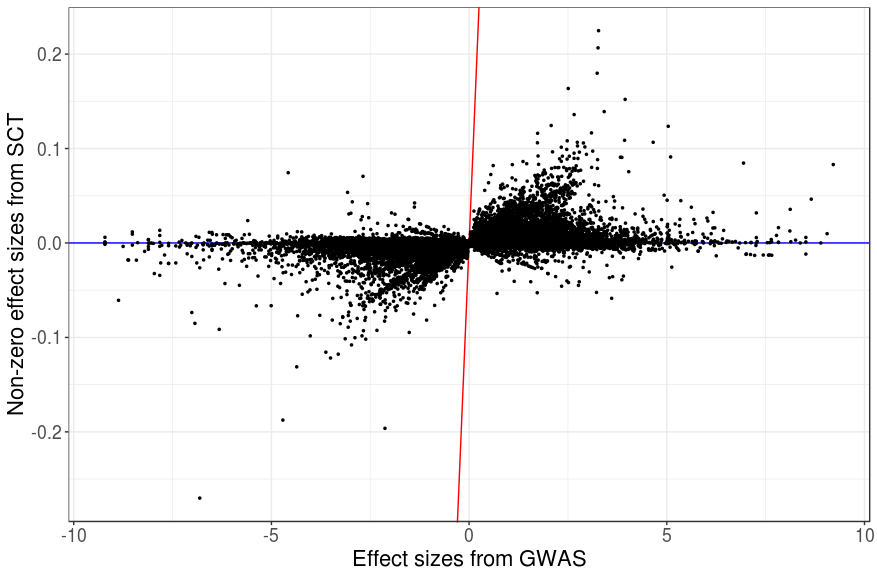
\includegraphics[width=\textwidth]{new-effects-MDD.png}
\caption{Depression}
\end{subfigure}
\end{figure}

\begin{figure}[htb]\ContinuedFloat
\centering
\begin{subfigure}[b]{0.7\textwidth}
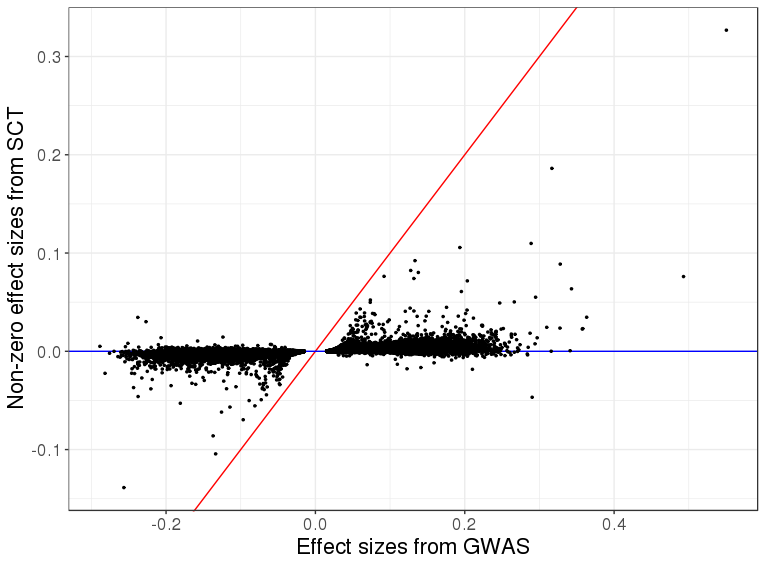
\includegraphics[width=\textwidth]{new-effects-CAD.png}
\caption{Coronary artery disease}
\end{subfigure}
\\~\\~\\
\begin{subfigure}[b]{0.7\textwidth}
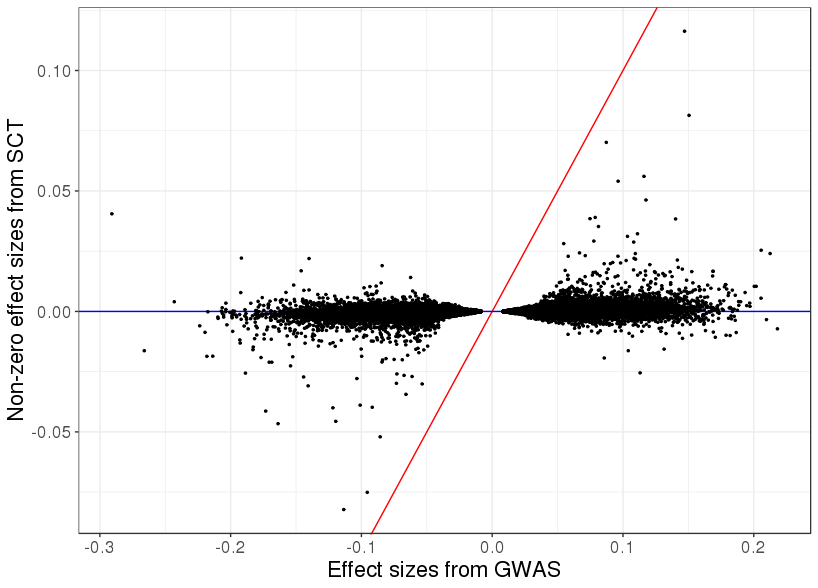
\includegraphics[width=\textwidth]{new-effects-asthma.png}
\caption{Asthma}
\end{subfigure}

\caption{New effect sizes resulting from SCT versus initial effect sizes of GWAS in real data applications. Only non-zero effects are represented. Red line corresponds to the 1:1 line.}
\label{fig:neweffreal}
\end{figure}

%%%%%%%%%%%%%%%%%%%%%%%%%%%%%%%%%%%%%%%%%%%%%%%%%%%%%%%%%%%%%%%%%%%%%%%%%%%%%%%%

\begin{figure}[htb]
\centering
\begin{subfigure}[b]{\textwidth}
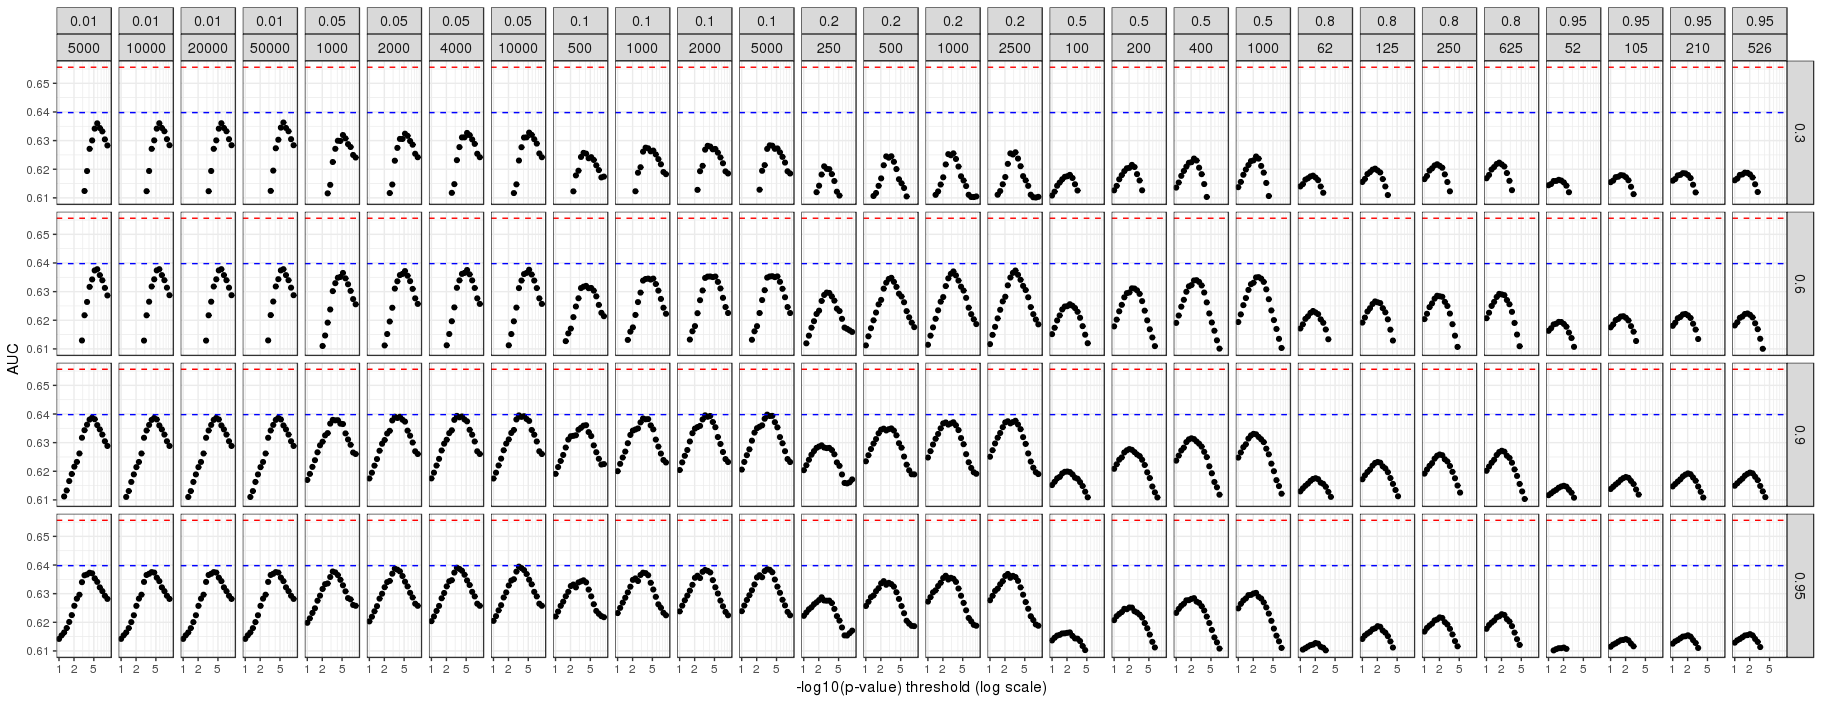
\includegraphics[width=\textwidth]{grid-BRCA.png}
\caption{Breast cancer}
\end{subfigure}
\\~\\
\begin{subfigure}[b]{\textwidth}
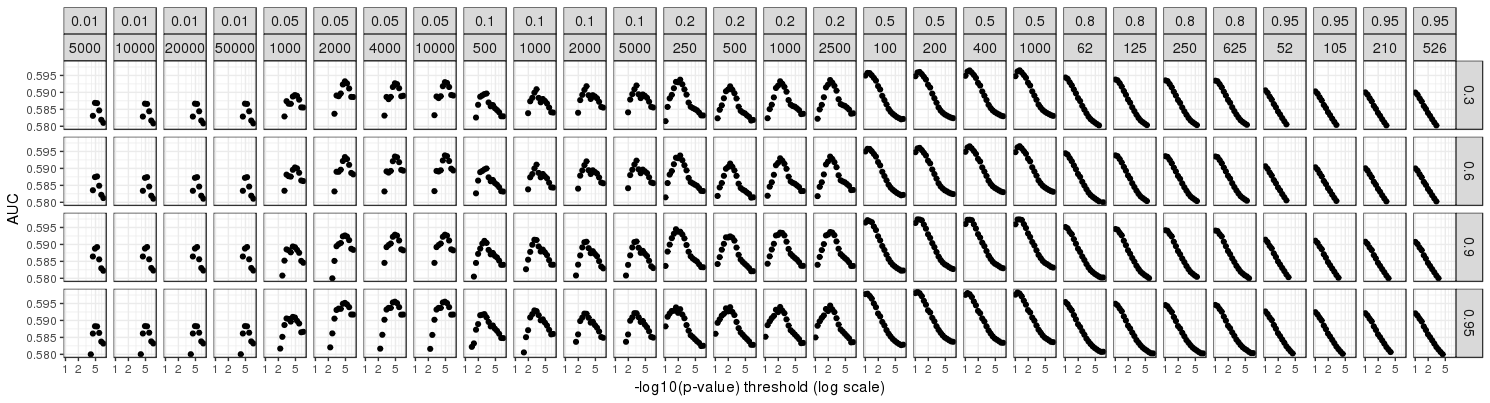
\includegraphics[width=\textwidth]{grid-RA.png}
\caption{Rheumatoid arthritis\label{fig:grid-RA}}
\end{subfigure}
\\~\\
\begin{subfigure}[b]{\textwidth}
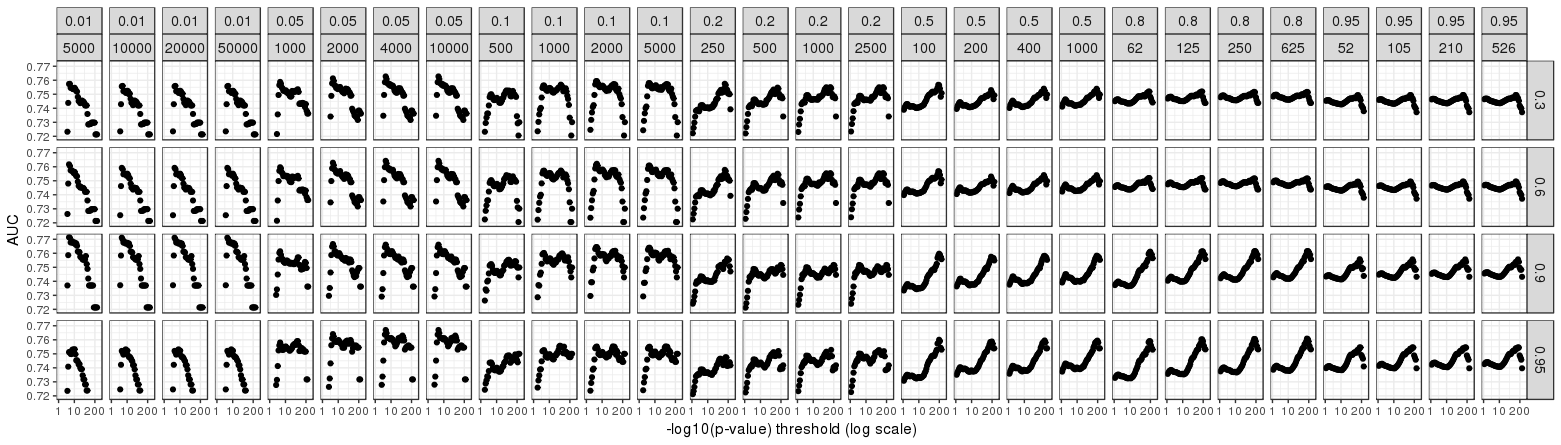
\includegraphics[width=\textwidth]{grid-T1D.png}
\caption{Type 1 diabetes}
\end{subfigure}
\end{figure}

\begin{figure}[htb]\ContinuedFloat
\centering
\begin{subfigure}[b]{\textwidth}
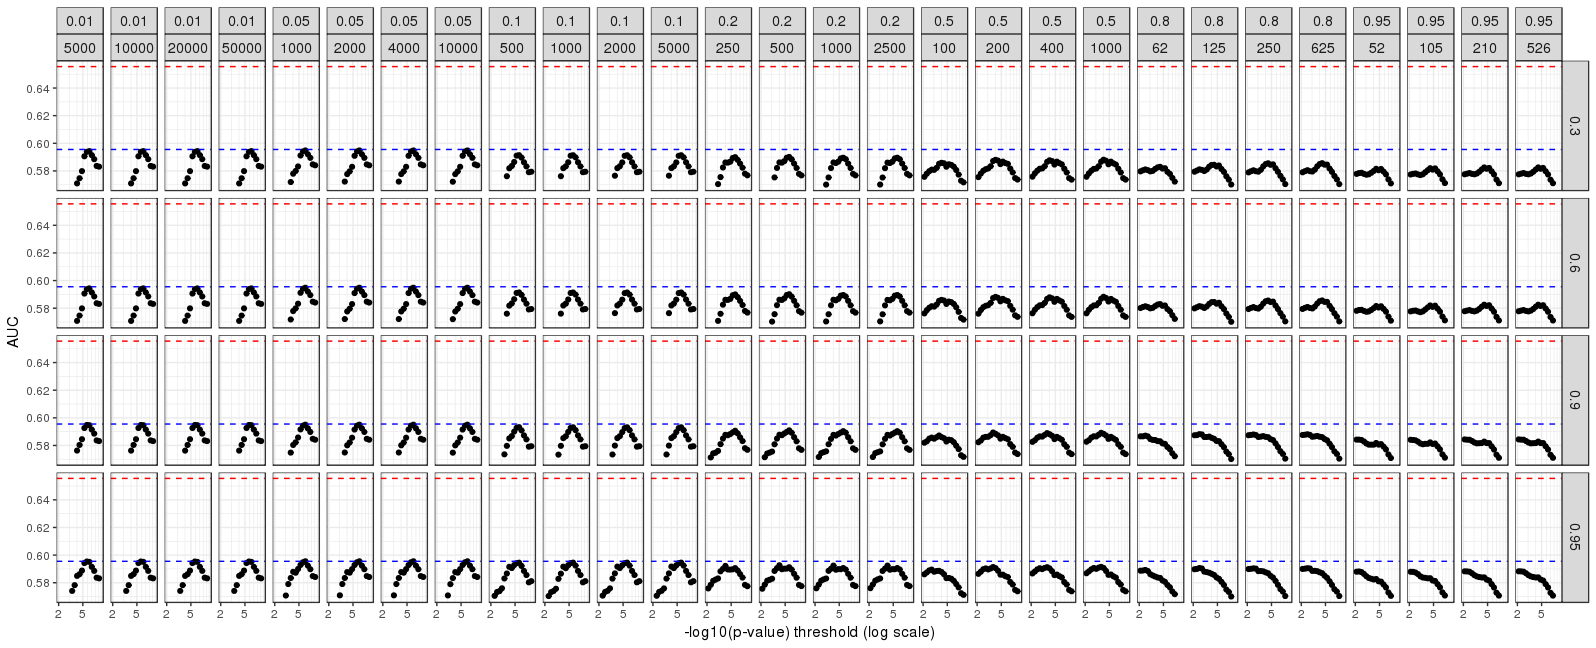
\includegraphics[width=\textwidth]{grid-T2D.png}
\caption{Type 2 diabetes}
\end{subfigure}
\\~\\
\begin{subfigure}[b]{\textwidth}
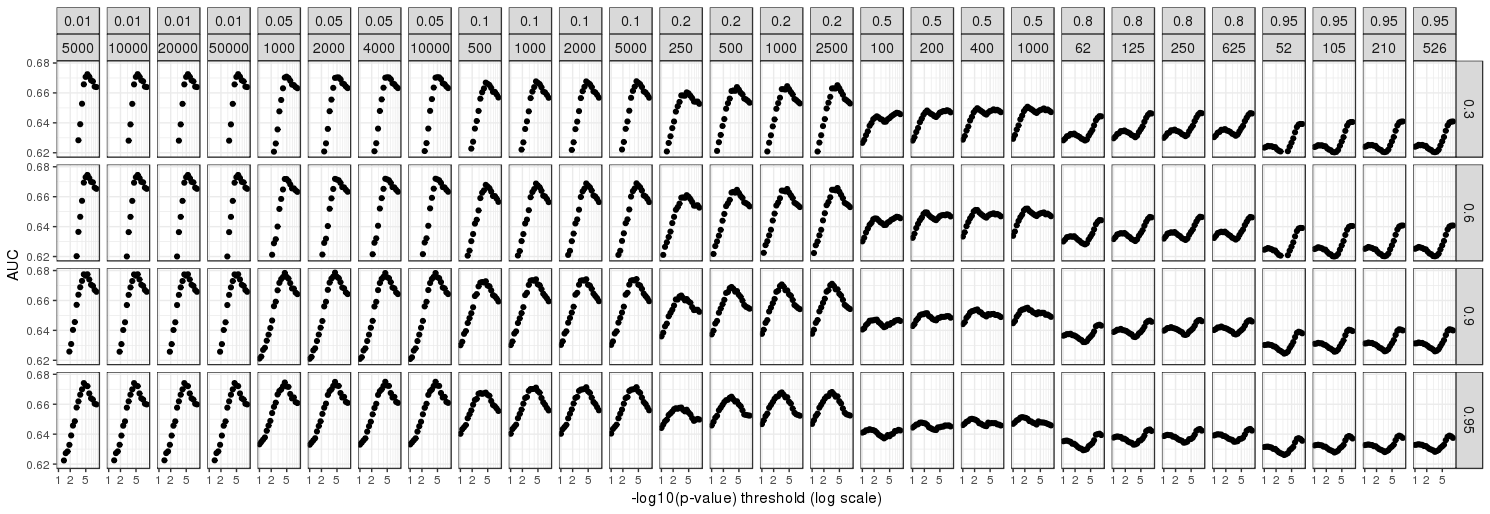
\includegraphics[width=\textwidth]{grid-PRCA.png}
\caption{Prostate cancer}
\end{subfigure}
\\~\\
\begin{subfigure}[b]{\textwidth}
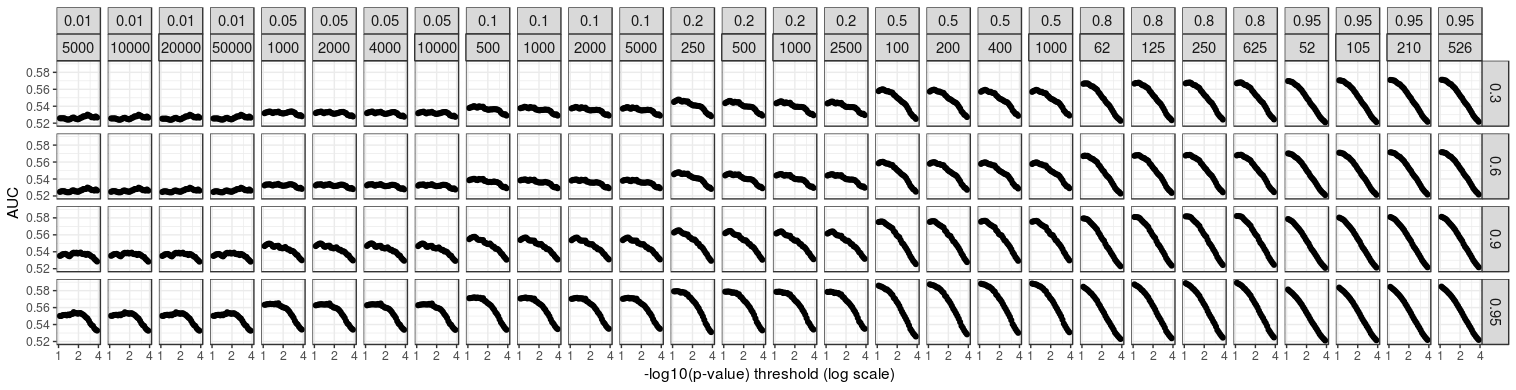
\includegraphics[width=\textwidth]{grid-MDD.png}
\caption{Depression\label{fig:grid-MDD}}
\end{subfigure}
\end{figure}

\begin{figure}[htb]\ContinuedFloat
\centering
\begin{subfigure}[b]{\textwidth}
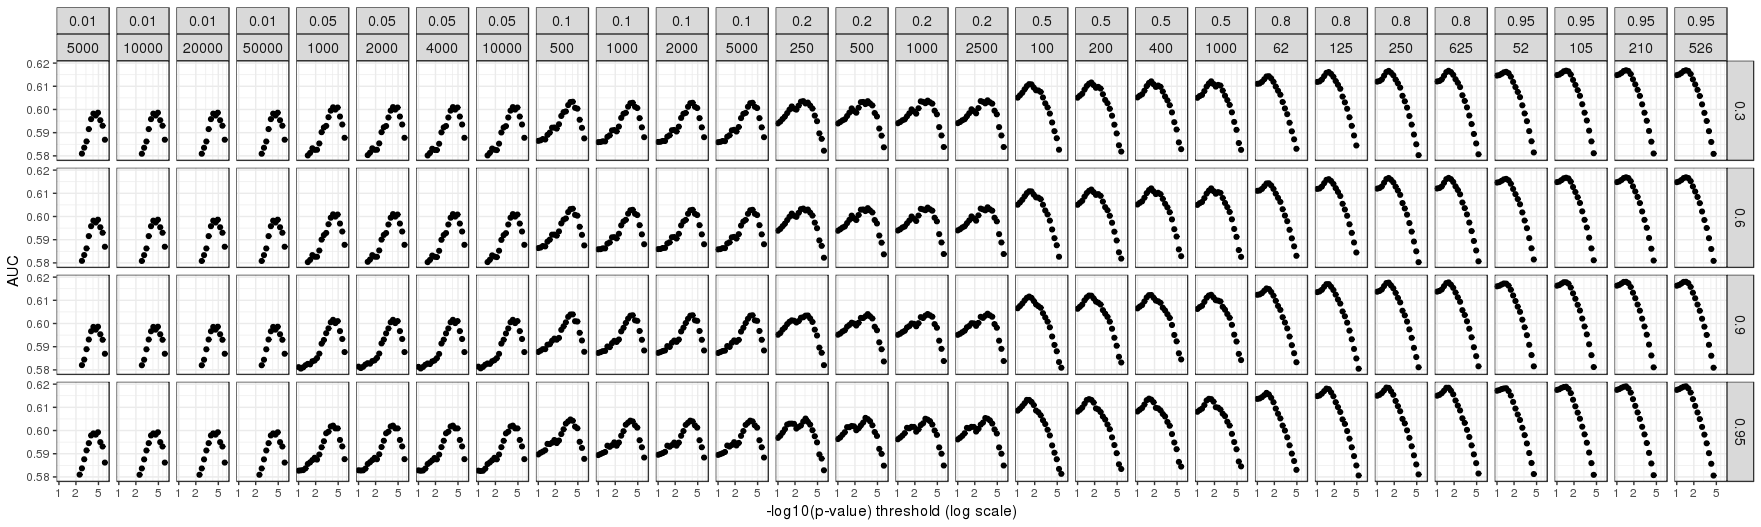
\includegraphics[width=\textwidth]{grid-CAD.png}
\caption{Coronary artery disease\label{fig:grid-CAD}}
\end{subfigure}
\\~\\
\begin{subfigure}[b]{\textwidth}
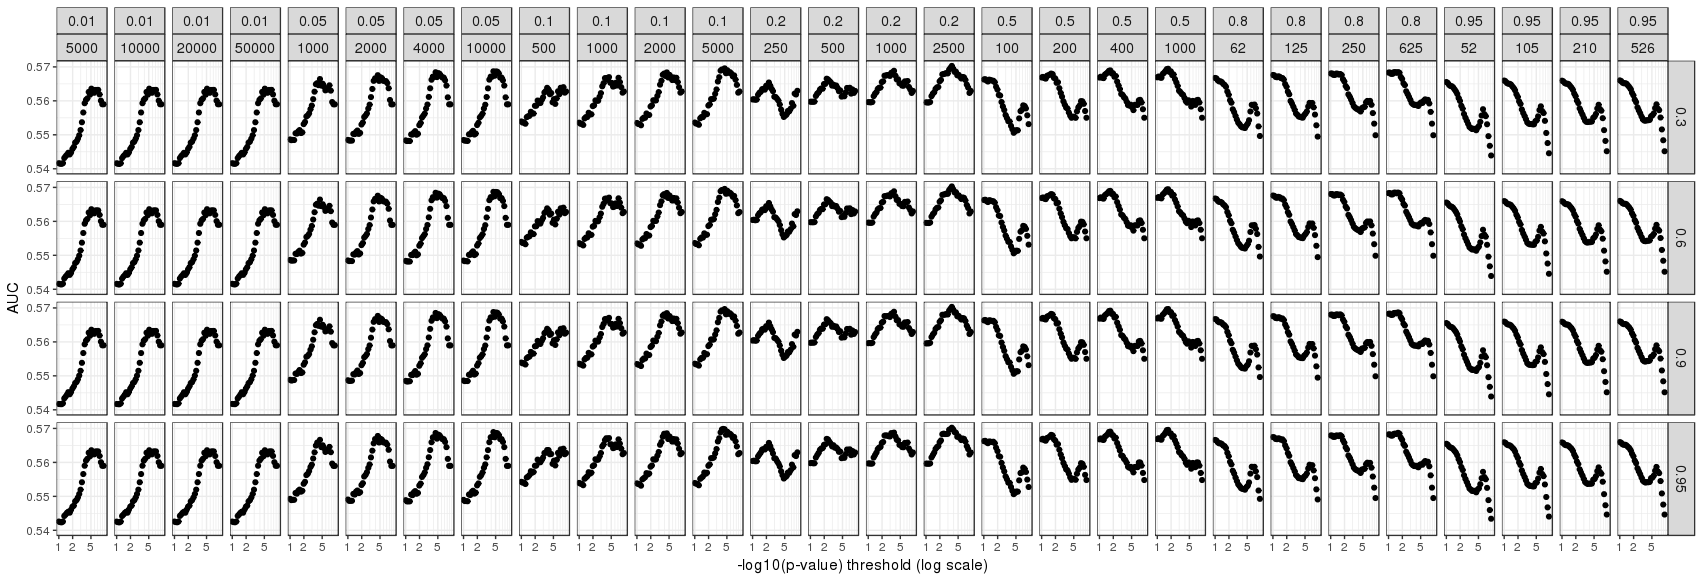
\includegraphics[width=\textwidth]{grid-asthma.png}
\caption{Asthma}
\end{subfigure}

\caption{AUC values (for the training set) when predicting disease status for many parameters of C+T in real data applications. Facets are presenting different clumping thresholds $r_c^2$ from 0.01 to 0.95, window sizes $w_c$ from 52 to 50,000 kb, and imputation thresholds from 0.3 to 0.95. The x-axis corresponds to the remaining hyper-parameter, the p-value threshold $p_T$; here, -log10(p-values) are represented using a logarithmic scale.}
\end{figure}

%%%%%%%%%%%%%%%%%%%%%%%%%%%%%%%%%%%%%%%%%%%%%%%%%%%%%%%%%%%%%%%%%%%%%%%%%%%%%%%%

\begin{figure}[htb]
\centerline{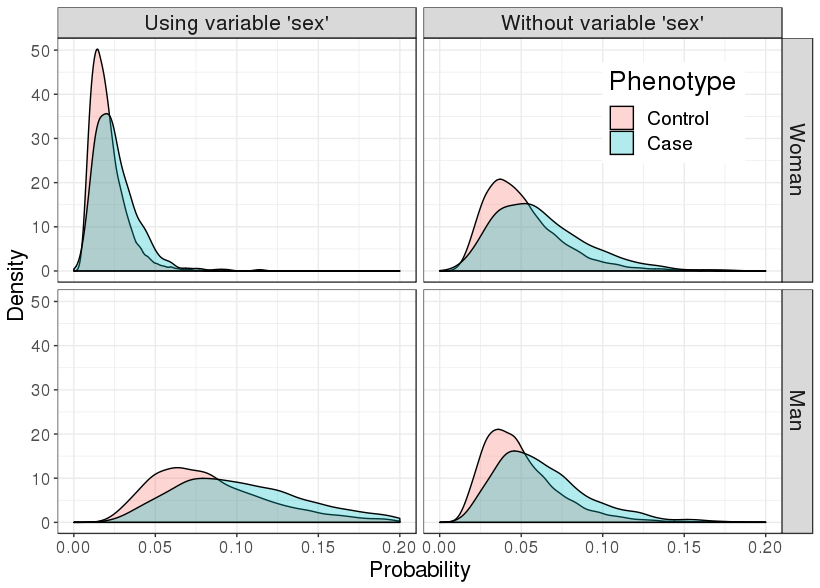
\includegraphics[width=0.8\textwidth]{dens-prob-CAD.png}}
\caption{Distribution of predicted probabilities of Coronary Artery Disease (CAD) in the UK Biobank using SCT. Upper / lower panels corresponds to women / men. Left panels correspond to a model using C+T scores and variable `sex' when fitting penalized logistic regression in the stacking step. Right panels correspond to performing stacking of C+T scores without using variable `sex'.}
\label{fig:sexCAD}
\end{figure}

\end{document}
